This chapter presents progress towards a search for exotic Higgs decays to two light scalars with unequal mass ($h \rightarrow a_1 a_2$) final states with bottom quarks and $\tau$ leptons, with plans to interpret the results in the context of Two Real Singlet Models (TRSMs), described in Section \ref{section:theory-TRSM}.  Compared to the symmetric decay scenario $h\rightarrow aa$ which has been studied in multiple final states at CMS with stringent limits set on the various 2HDM+S scenarios, this asymmetric decay scenario has not been directly searched for at the CMS experiment. Section \ref{section:a1a2_masses} lists the mass hypotheses of the new particles $a_1$ and $a_2$ that will be studied. Section \ref{section:a1a2_gen_studies} describes the studies on which channels the analysis will be carried out in. Section \ref{section:a1a2_control_plots} shows the control plots produced using the analysis framework that will be used for this analysis.

\section{Signal masses}
\label{section:a1a2_masses}
As discussed in Section \ref{section:theory-TRSM}, $h \rightarrow a_1 a_2$ can result in a ``cascade" decay if one of the scalars, $a_2$ is sufficiently heavy ($m_{a_2} > 2m_{a_1}$). The ``non-cascade" case is where the light scalars decay directly to Standard Model particles. 

The mass hypotheses (mass points) $(m_{a_1}, m_{a_2})$ studied here are:
\begin{itemize}
    \item \textit{Cascade mass points:} (15, 30), (15, 40), (15, 50), (15, 60), (15, 70), (15, 80), (15, 90), (15, 100), (15, 110), (20, 40), (20, 50), (20, 60), (20, 70), (20, 80), (20, 90), (20, 100), (30, 60), (30, 70), (30, 80), and (30, 90) GeV
    \item \textit{Non-cascade mass points:} (15, 20), (15, 30), (20, 30), (20, 40), (30, 40), (30, 50), (30, 60), (40, 50), (40, 60), (40, 70), (40, 80), (50, 60), and (50, 70) GeV
\end{itemize}
Samples were produced using the MadGraph5\_aMCatNLO event generator, for each signal mass point in the gluon-gluon fusion (ggF) and vector boson fusion (VBF) production modes of the 125 GeV Higgs boson. In the sample generation, the decays of $a$ to Standard Model particles were specified to be decays to bottom quarks or $\tau$ leptons.


\section{Cascade scenario signal studies}
\label{section:a1a2_gen_studies}
Studies of the signal phenomenology in the cascade scenario were performed to determine the viability of the $4b2\tau$ and/or $2b4\tau$ channels. 

Cross sections and branching fractions of the $4b2\tau$ and $2b4\tau$ final states were compared using cross-section predictions provided by the authors of \cite{Robens:2019kga}. For an example mass point $m_{a_2} = 80$ GeV, $m_{a_1} = 30$ GeV, the branching fractions to $4b2\tau$ is ten times larger than $2b4\tau$: $B(h \rightarrow a_1 a_2 \rightarrow 3 a_1 \rightarrow 4b2\tau) = 0.00857$, vs. $B(h \rightarrow a_1 a_2 \rightarrow 3 a_1 \rightarrow 2b4\tau) = 0.00068$. The $4b2\tau$ final state is chosen for this analysis.

In general the four b-flavor jets have low $p_{T}$ at generator level, as illustrated for example mass points (100, 15) GeV and (40, 20) GeV in Fig. \ref{fig:overlay_cascade_b_jet_gen_pT}. The $p_{T}$ distribution of the sub-leading jet peaks at an energy below 20 GeV, with the third and fourth jets tending to have even softer energies.

An event category with three or more b-tag jets was determined to be infeasible due to low statistics in this category, due to the difficulties in reconstructing the third and fourth b-flavor jets which have very low transverse momenta $p_{T}$. Event categories with exactly 1 b-tag jet and $\geq 2$ b-tag jets will be used.

\begin{figure}[ht]
    \centering
    \begin{subfigure}{0.45\textwidth}
        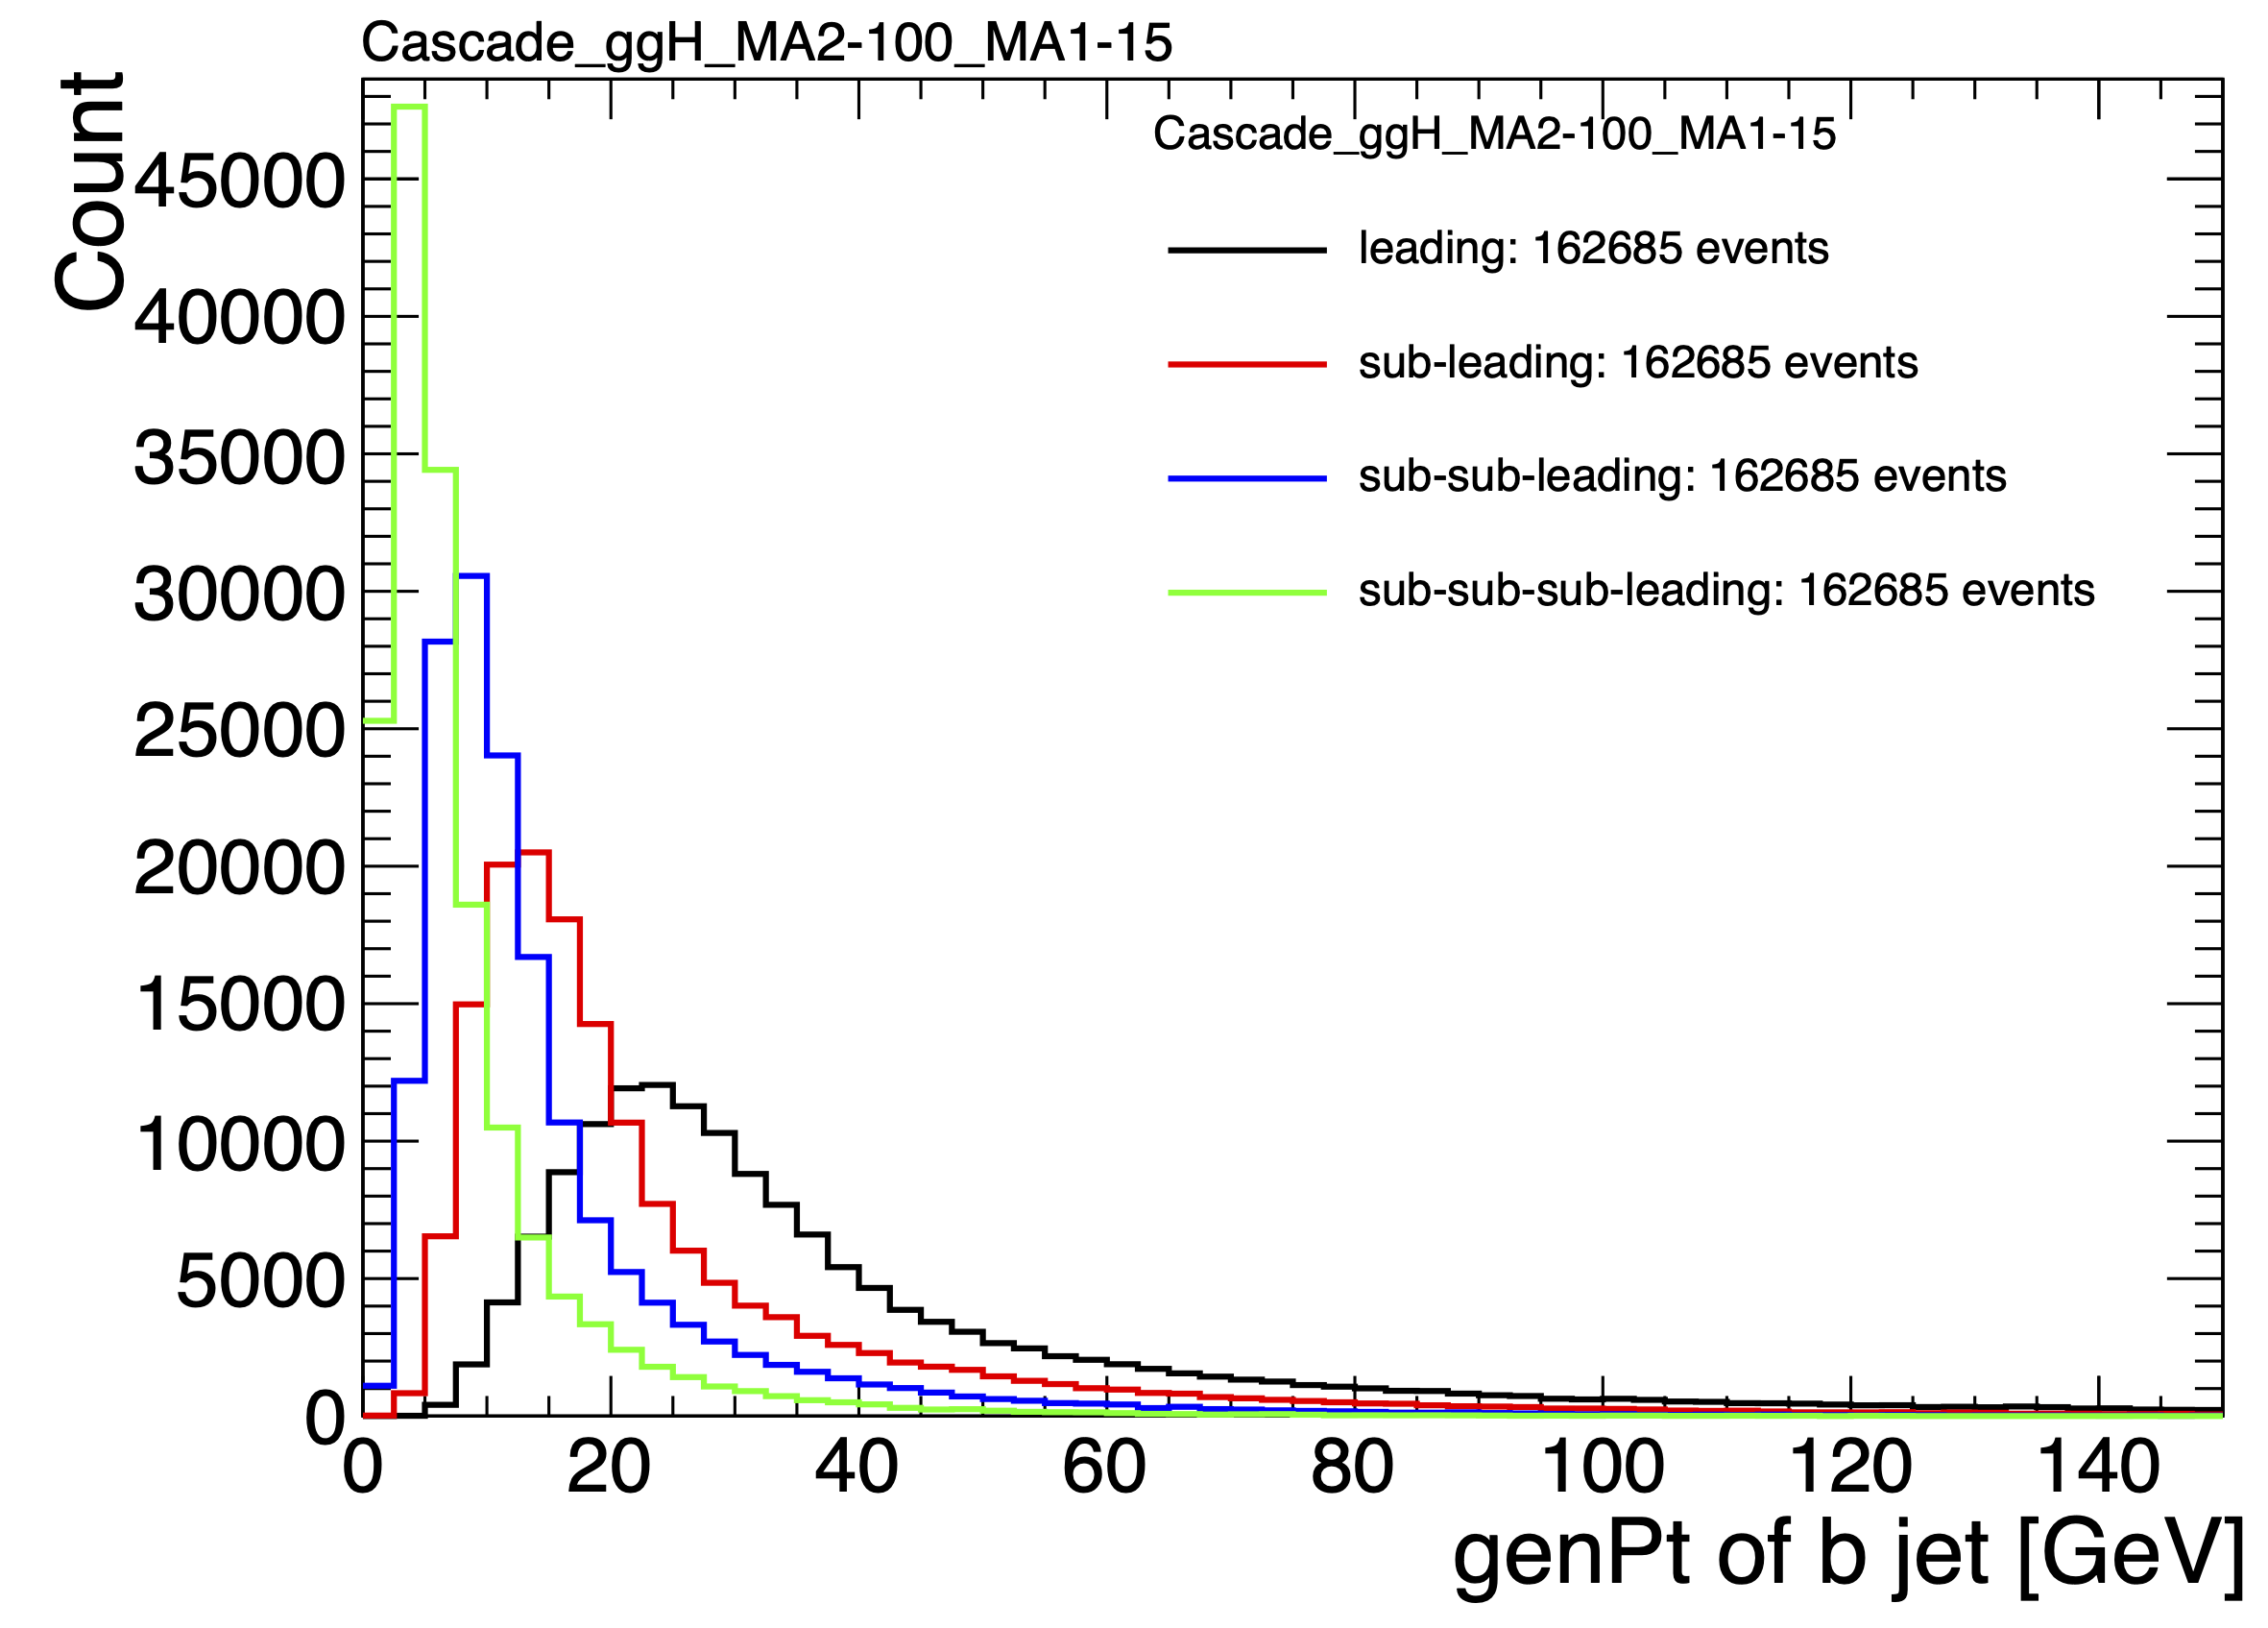
\includegraphics[width=1.0\textwidth]{figures/ch-11-asymmetric/Cascade_ggH_MA2-100_MA1-15_overlay}
    \end{subfigure}
    \hfill
    \begin{subfigure}{0.45\textwidth}
        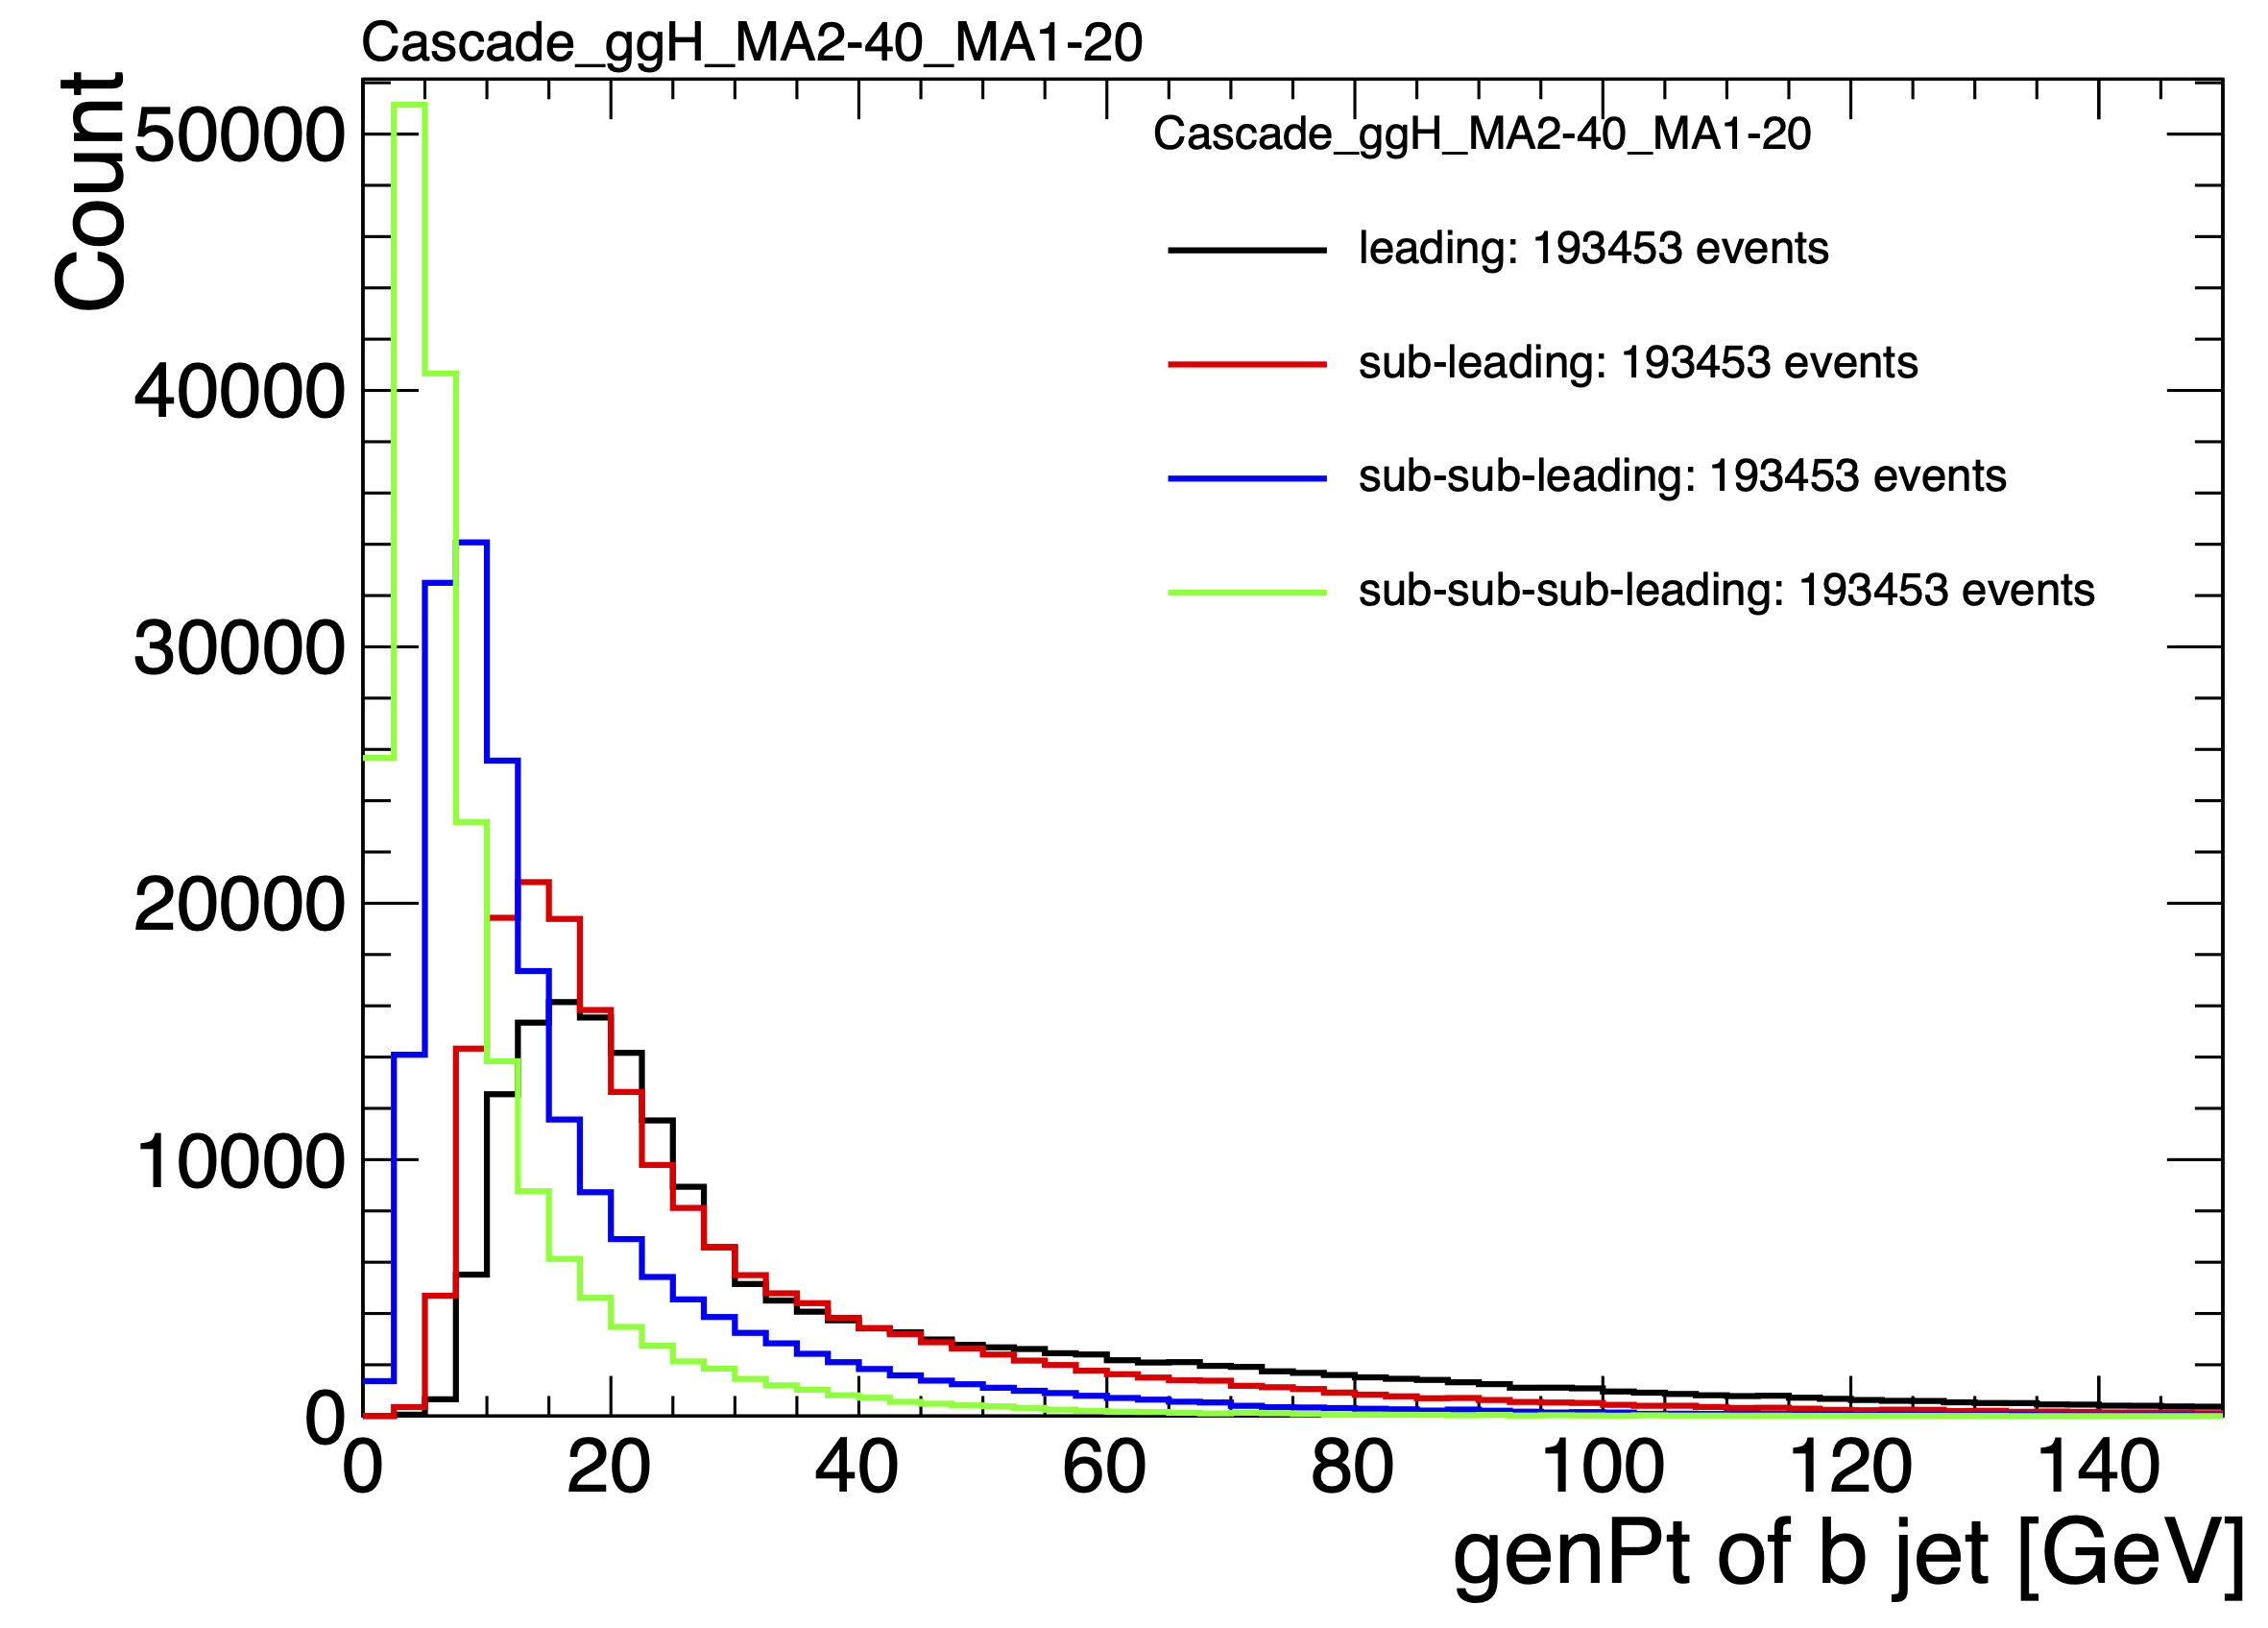
\includegraphics[width=1.0\textwidth]{figures/ch-11-asymmetric/Cascade_ggH_MA2-40_MA1-20_overlay}
    \end{subfigure}  
    \caption{Generator-level b-flavor jet transverse momenta $p_{T}$, for $h \rightarrow a_1 a_2$ cascade scenario in the $4b2\tau$ final state, for mass hypotheses $(m_{a_1}, m_{a_2}) = (100, 15)$ GeV (\textit{left}) and (40, 20) GeV (\textit{right}). In each plot the generator-level $p_{T}$ of the leading (\textit{black}), sub-leading (\textit{red}), third (\textit{blue}), and fourth (\textit{light green}) are overlaid.}
    \label{fig:overlay_cascade_b_jet_gen_pT}
\end{figure}


In the $4b2\tau$ final state, the possibility of the leading and sub-leading b-tag jets being sufficiently close in $\Delta R$ to require boosted jet reconstruction techniques was explored. In the $4b2\tau$ case, the two b-flavor-jets in the generated event that were spatially closest in $\Delta R$ were considered as one object. This two b-flavor jet object was spatially matched in $\Delta R$ to the jets reconstructed with the standard AK4 algorithm which uses a cone size of $\Delta R = 0.4$. The quality of the $p_{T}$ resolution (computed as $(p_{T, \text{reconstructed}} - p_{T, \text{gen}})/ p_{T, \text{gen}}$) and closeness in distance $\Delta R$ of the reconstructed jet to the nearest generator-level jets, was seen to depend on the absolute and relative masses of the light scalars. The best (worst) performance occurred in samples with large (small) mass differences between the heavier scalar $a_2$ and the lighter scalar $a_1$, as illustrated for the mass hypotheses $(m_{a_1}, m_{a_2})$ (100, 15) GeV and (40, 20) GeV in Fig. \ref{fig:cascade_matching_to_AK4_jets}.


\begin{figure}[ht]
    \centering
    \begin{subfigure}{0.45\textwidth}
        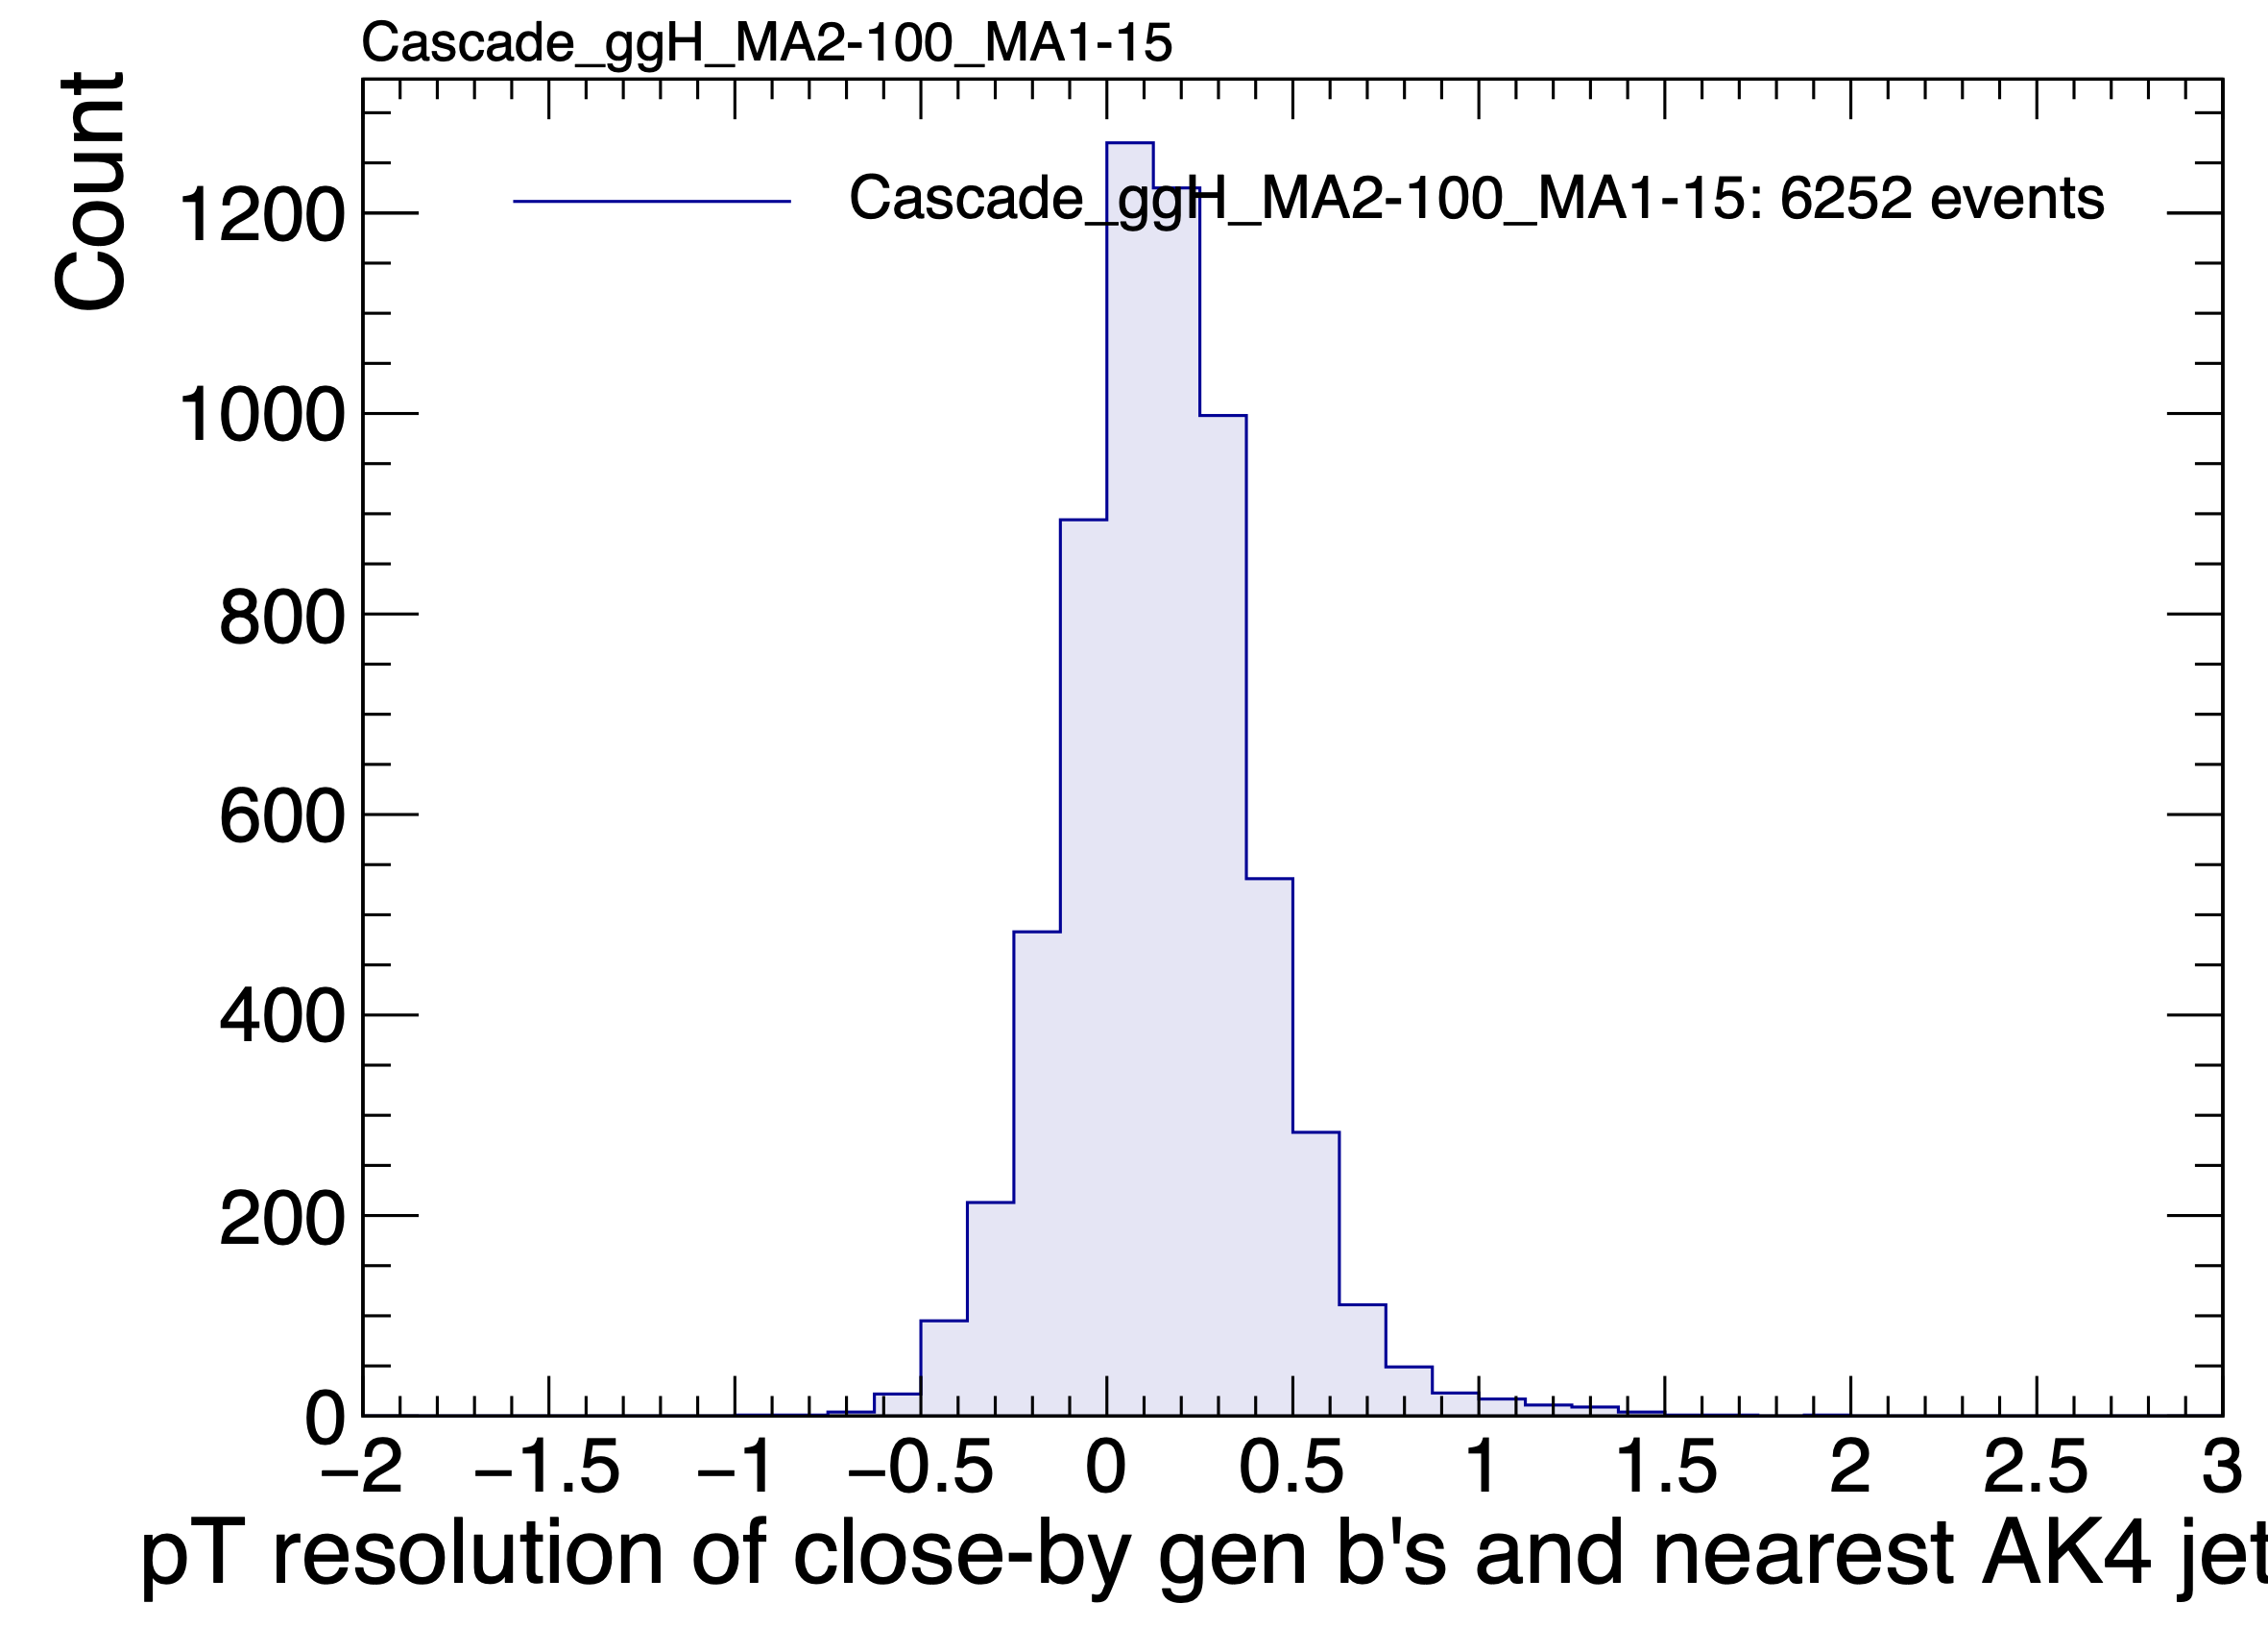
\includegraphics[width=1.0\textwidth]{figures/ch-11-asymmetric/Cascade_ggH_MA2-100_MA1-15_pt_resolution_ak4_leadingPair}
    \end{subfigure}
    \hfill
    \begin{subfigure}{0.45\textwidth}
        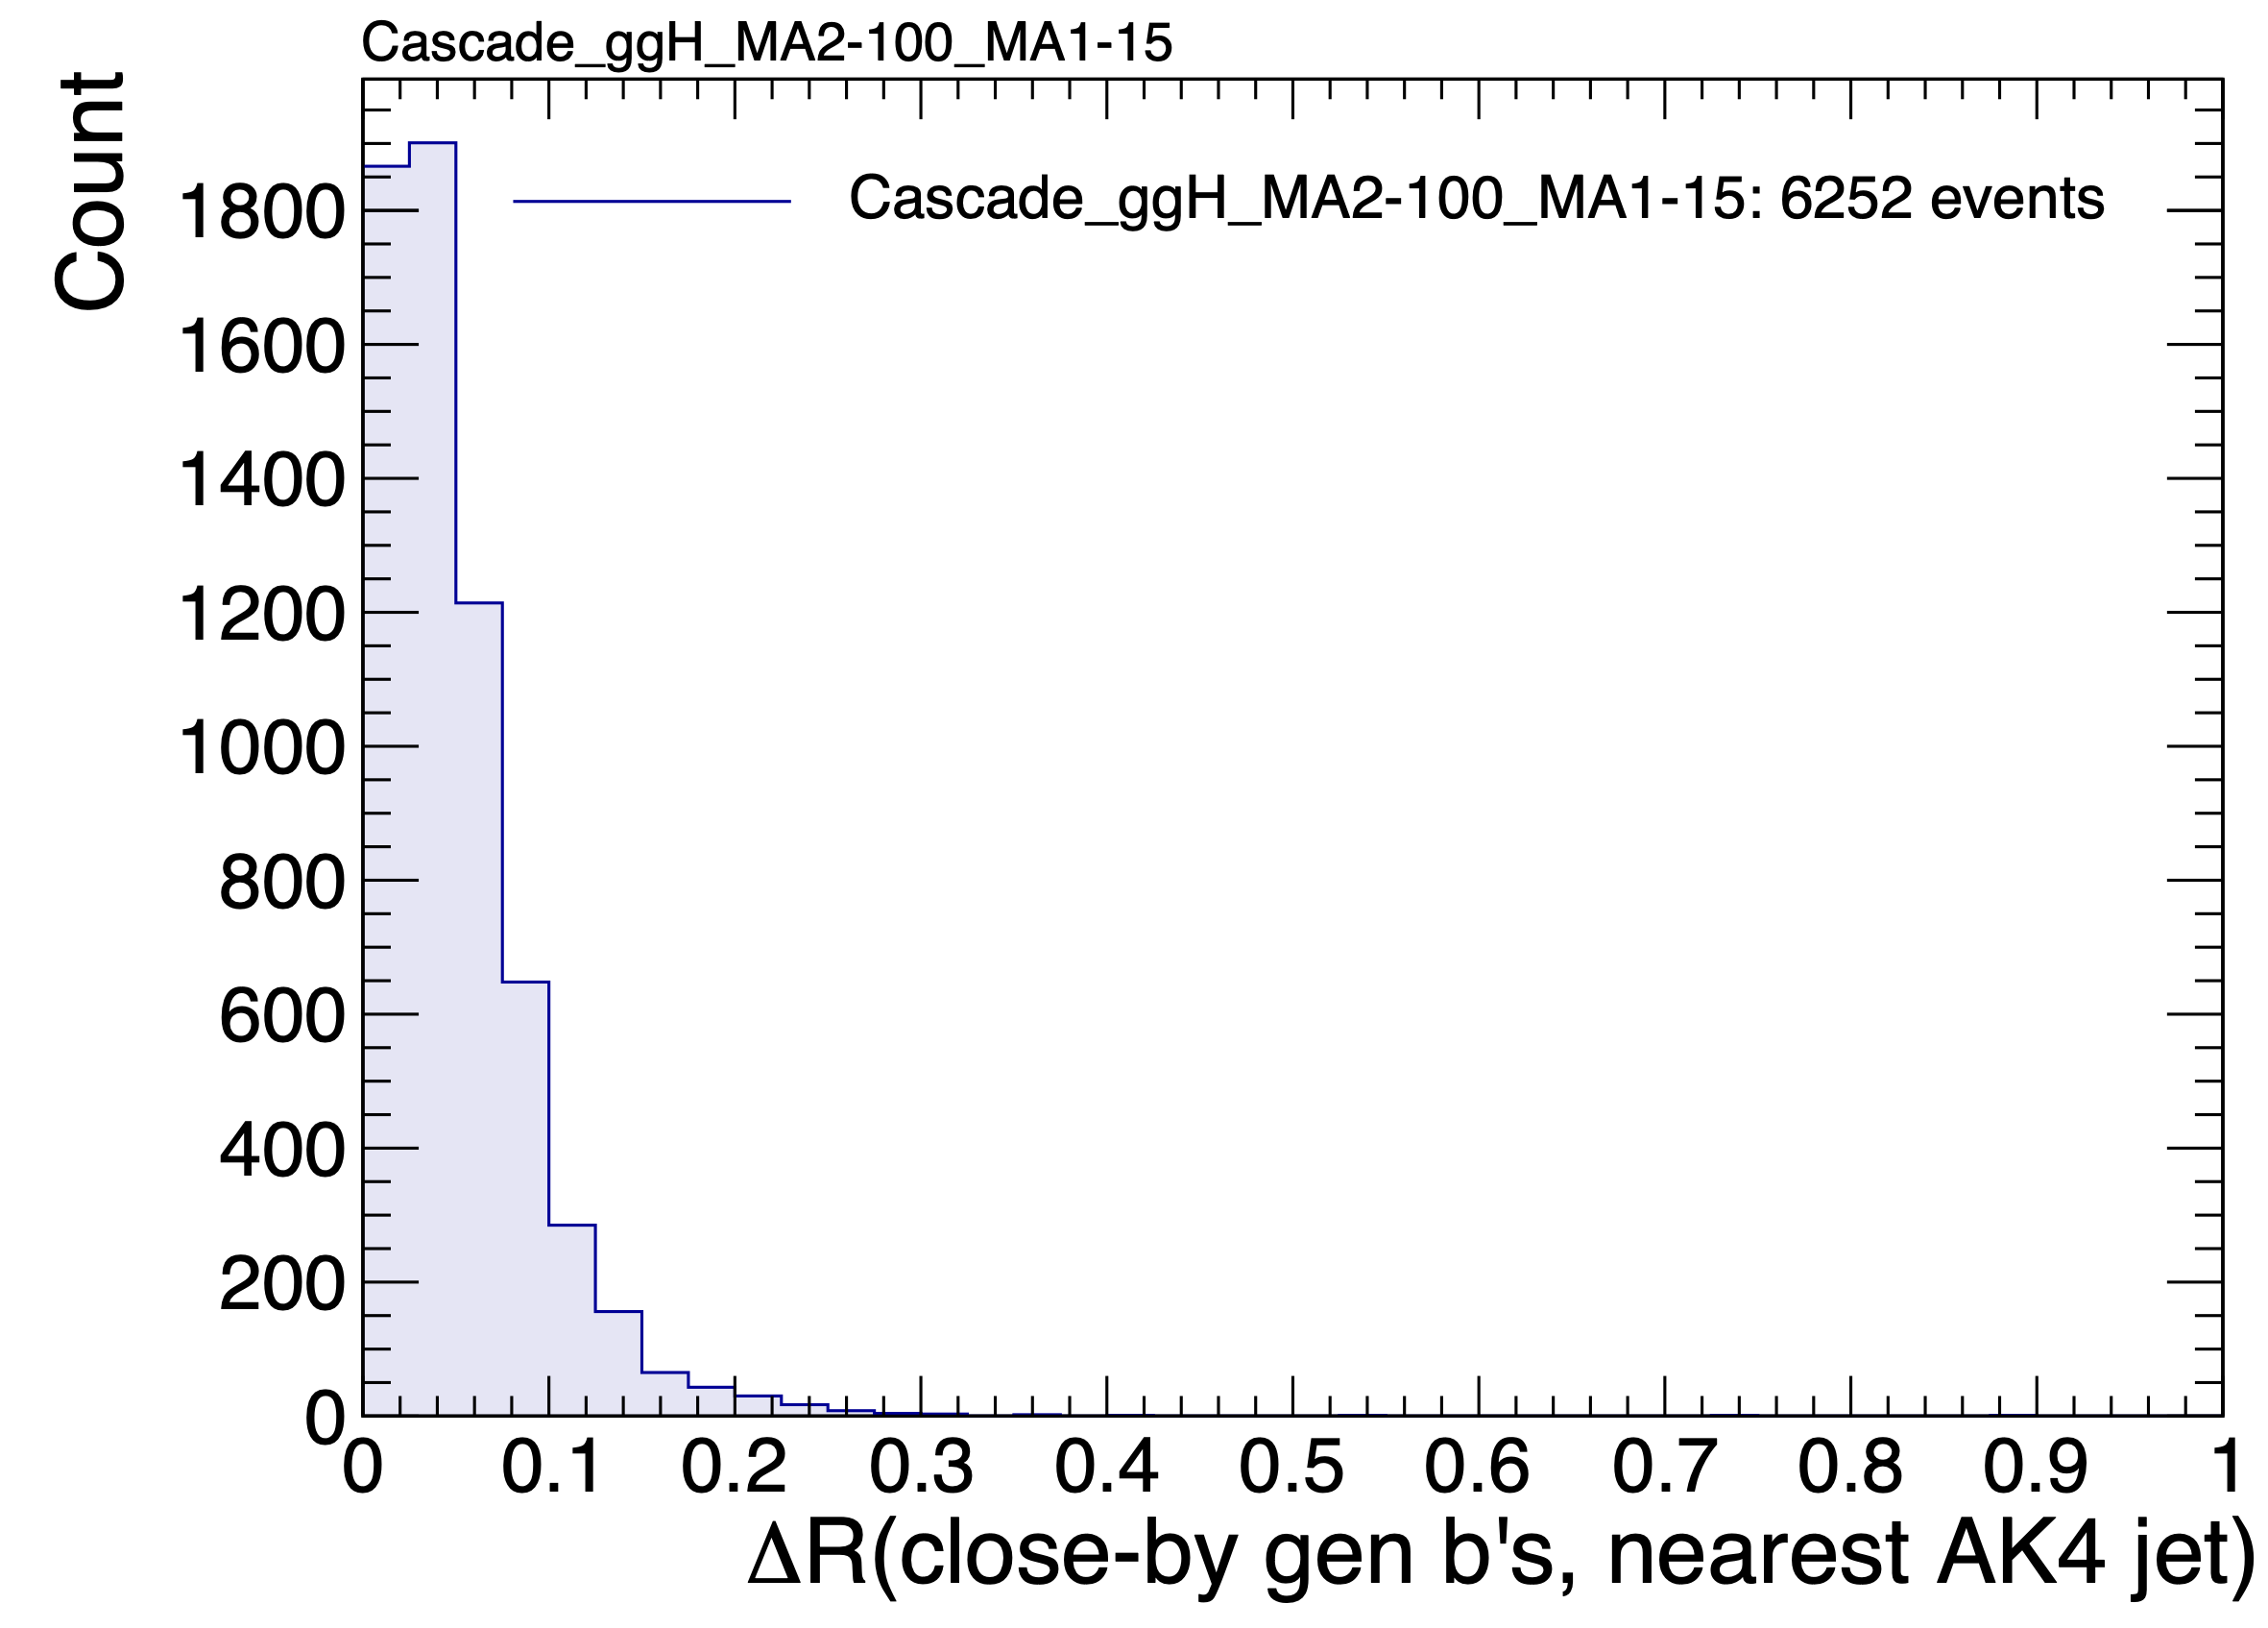
\includegraphics[width=1.0\textwidth]{figures/ch-11-asymmetric/Cascade_ggH_MA2-100_MA1-15_deltaR_ak4_leadingPair}
    \end{subfigure} \\
    \begin{subfigure}{0.45\textwidth}
        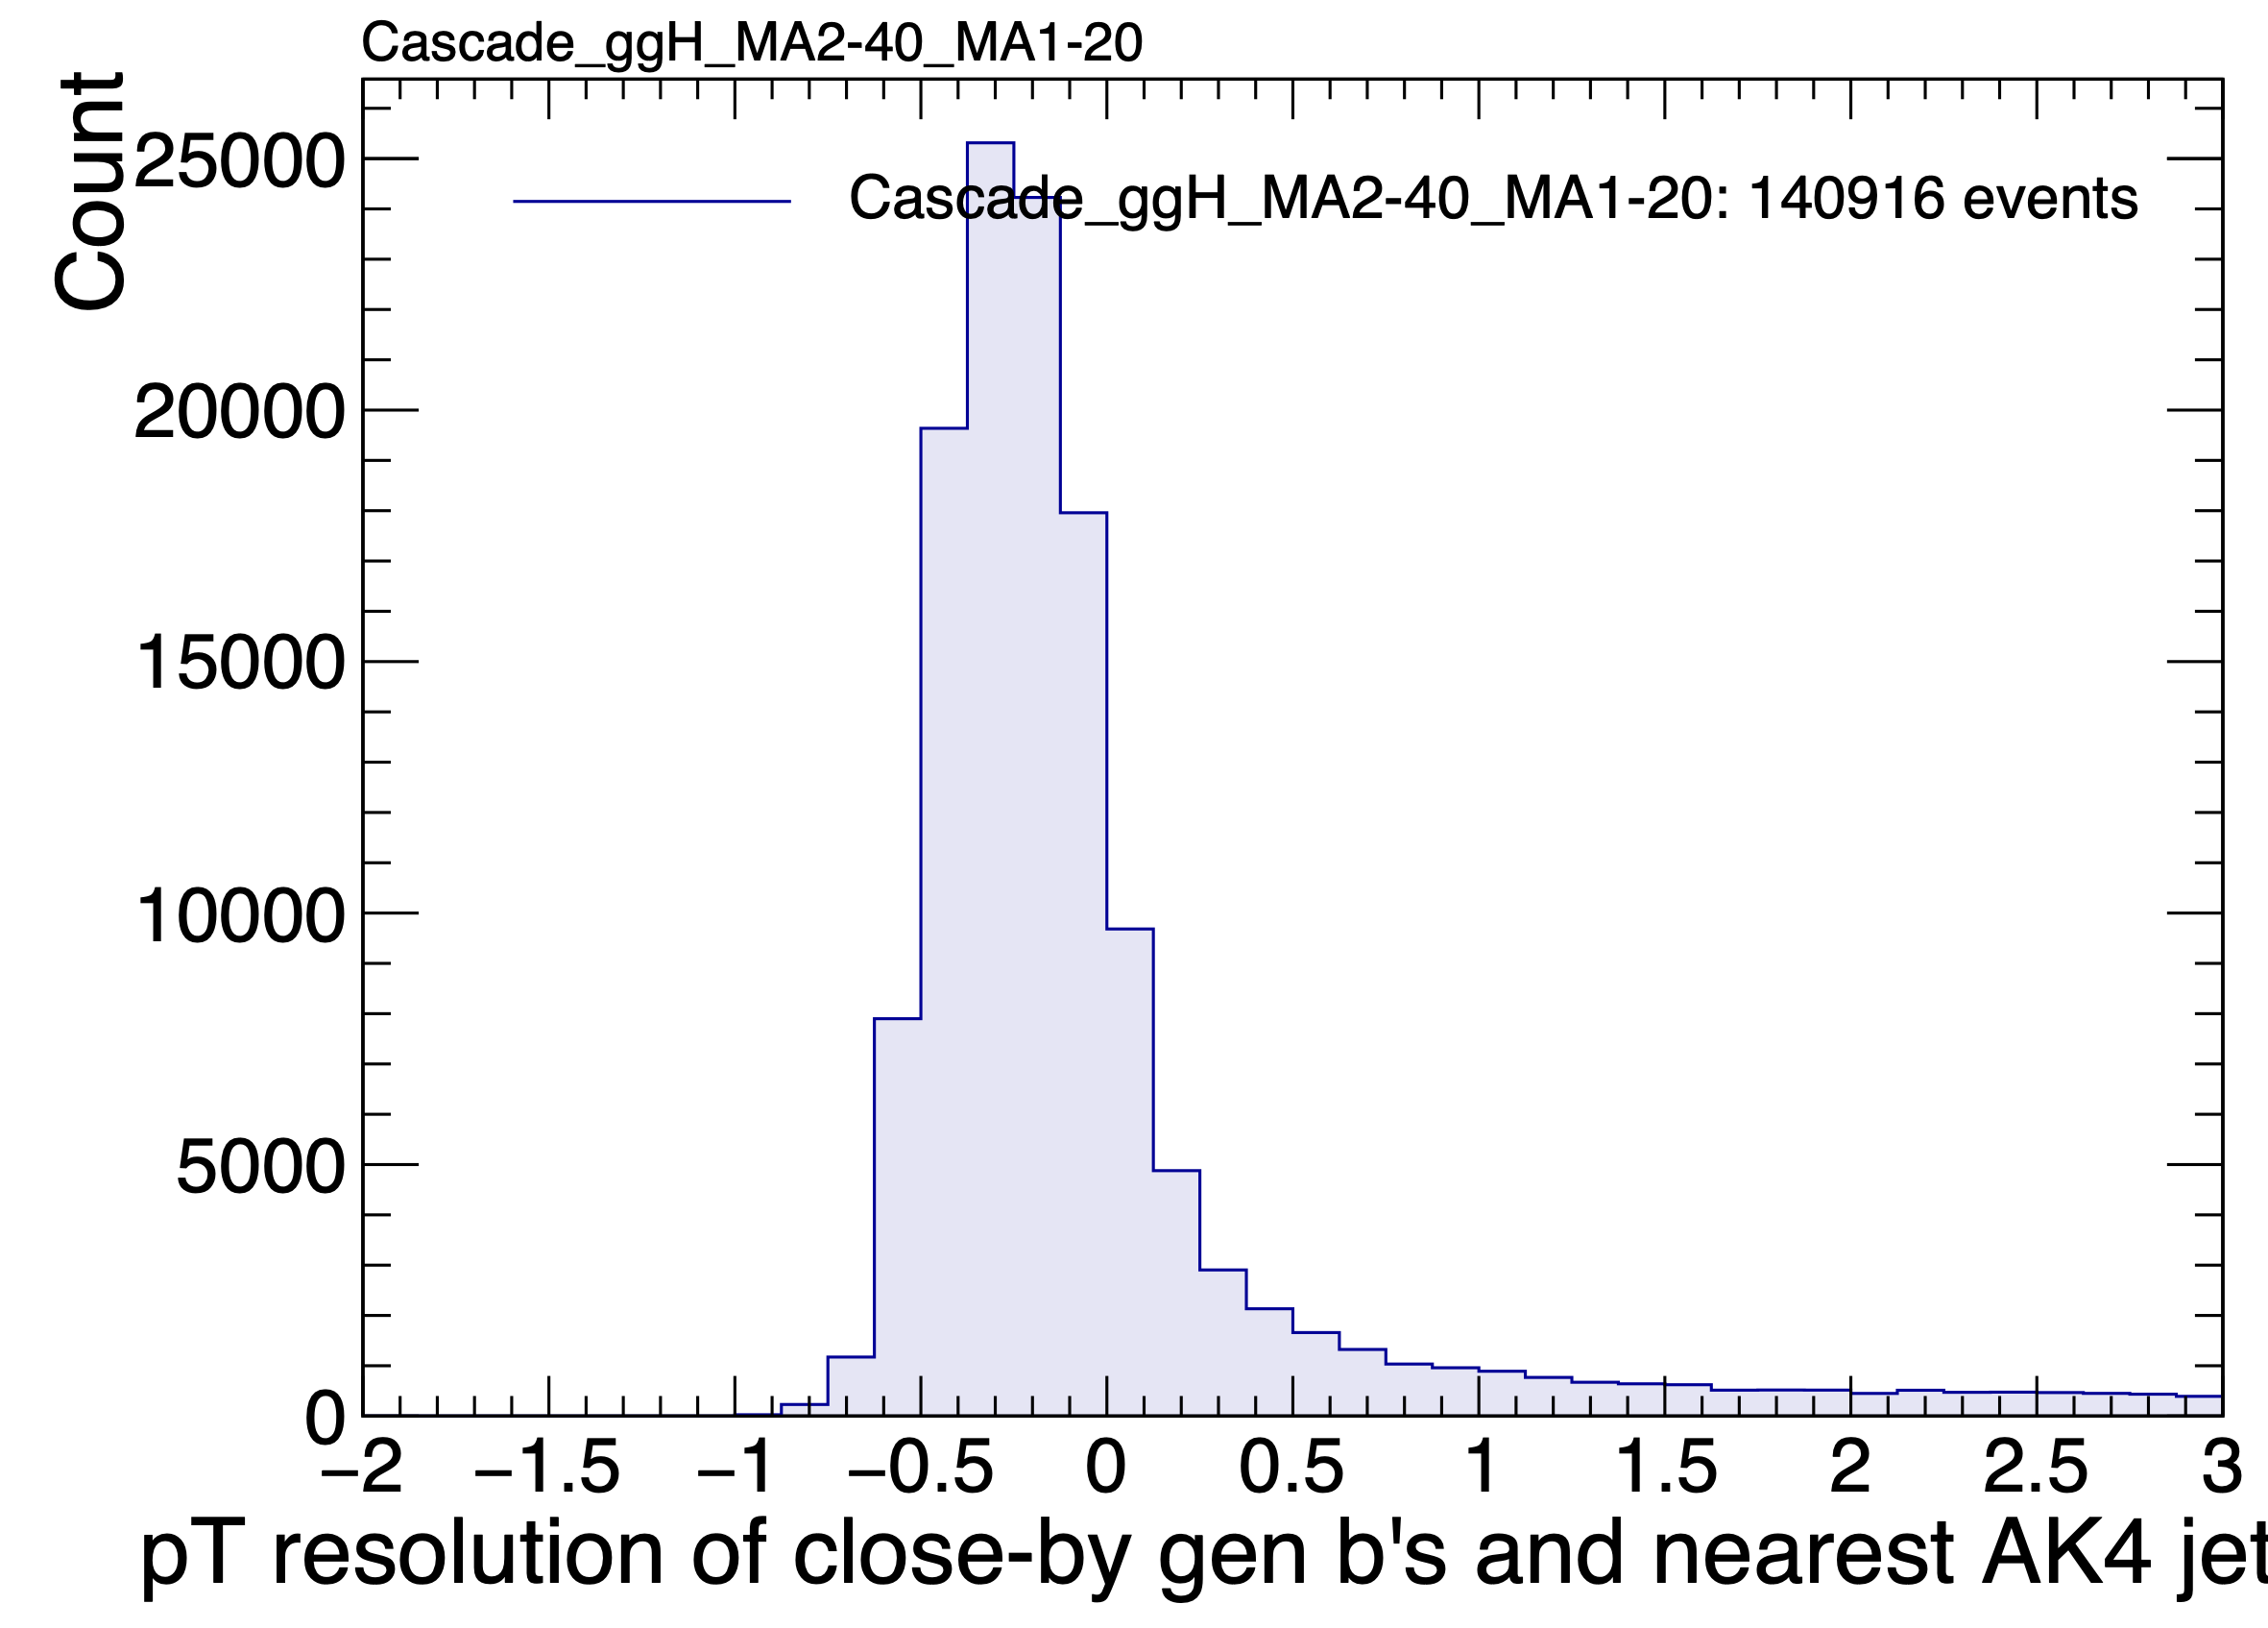
\includegraphics[width=1.0\textwidth]{figures/ch-11-asymmetric/Cascade_ggH_MA2-40_MA1-20_pt_resolution_ak4_leadingPair}
    \end{subfigure}
    \hfill
    \begin{subfigure}{0.45\textwidth}
        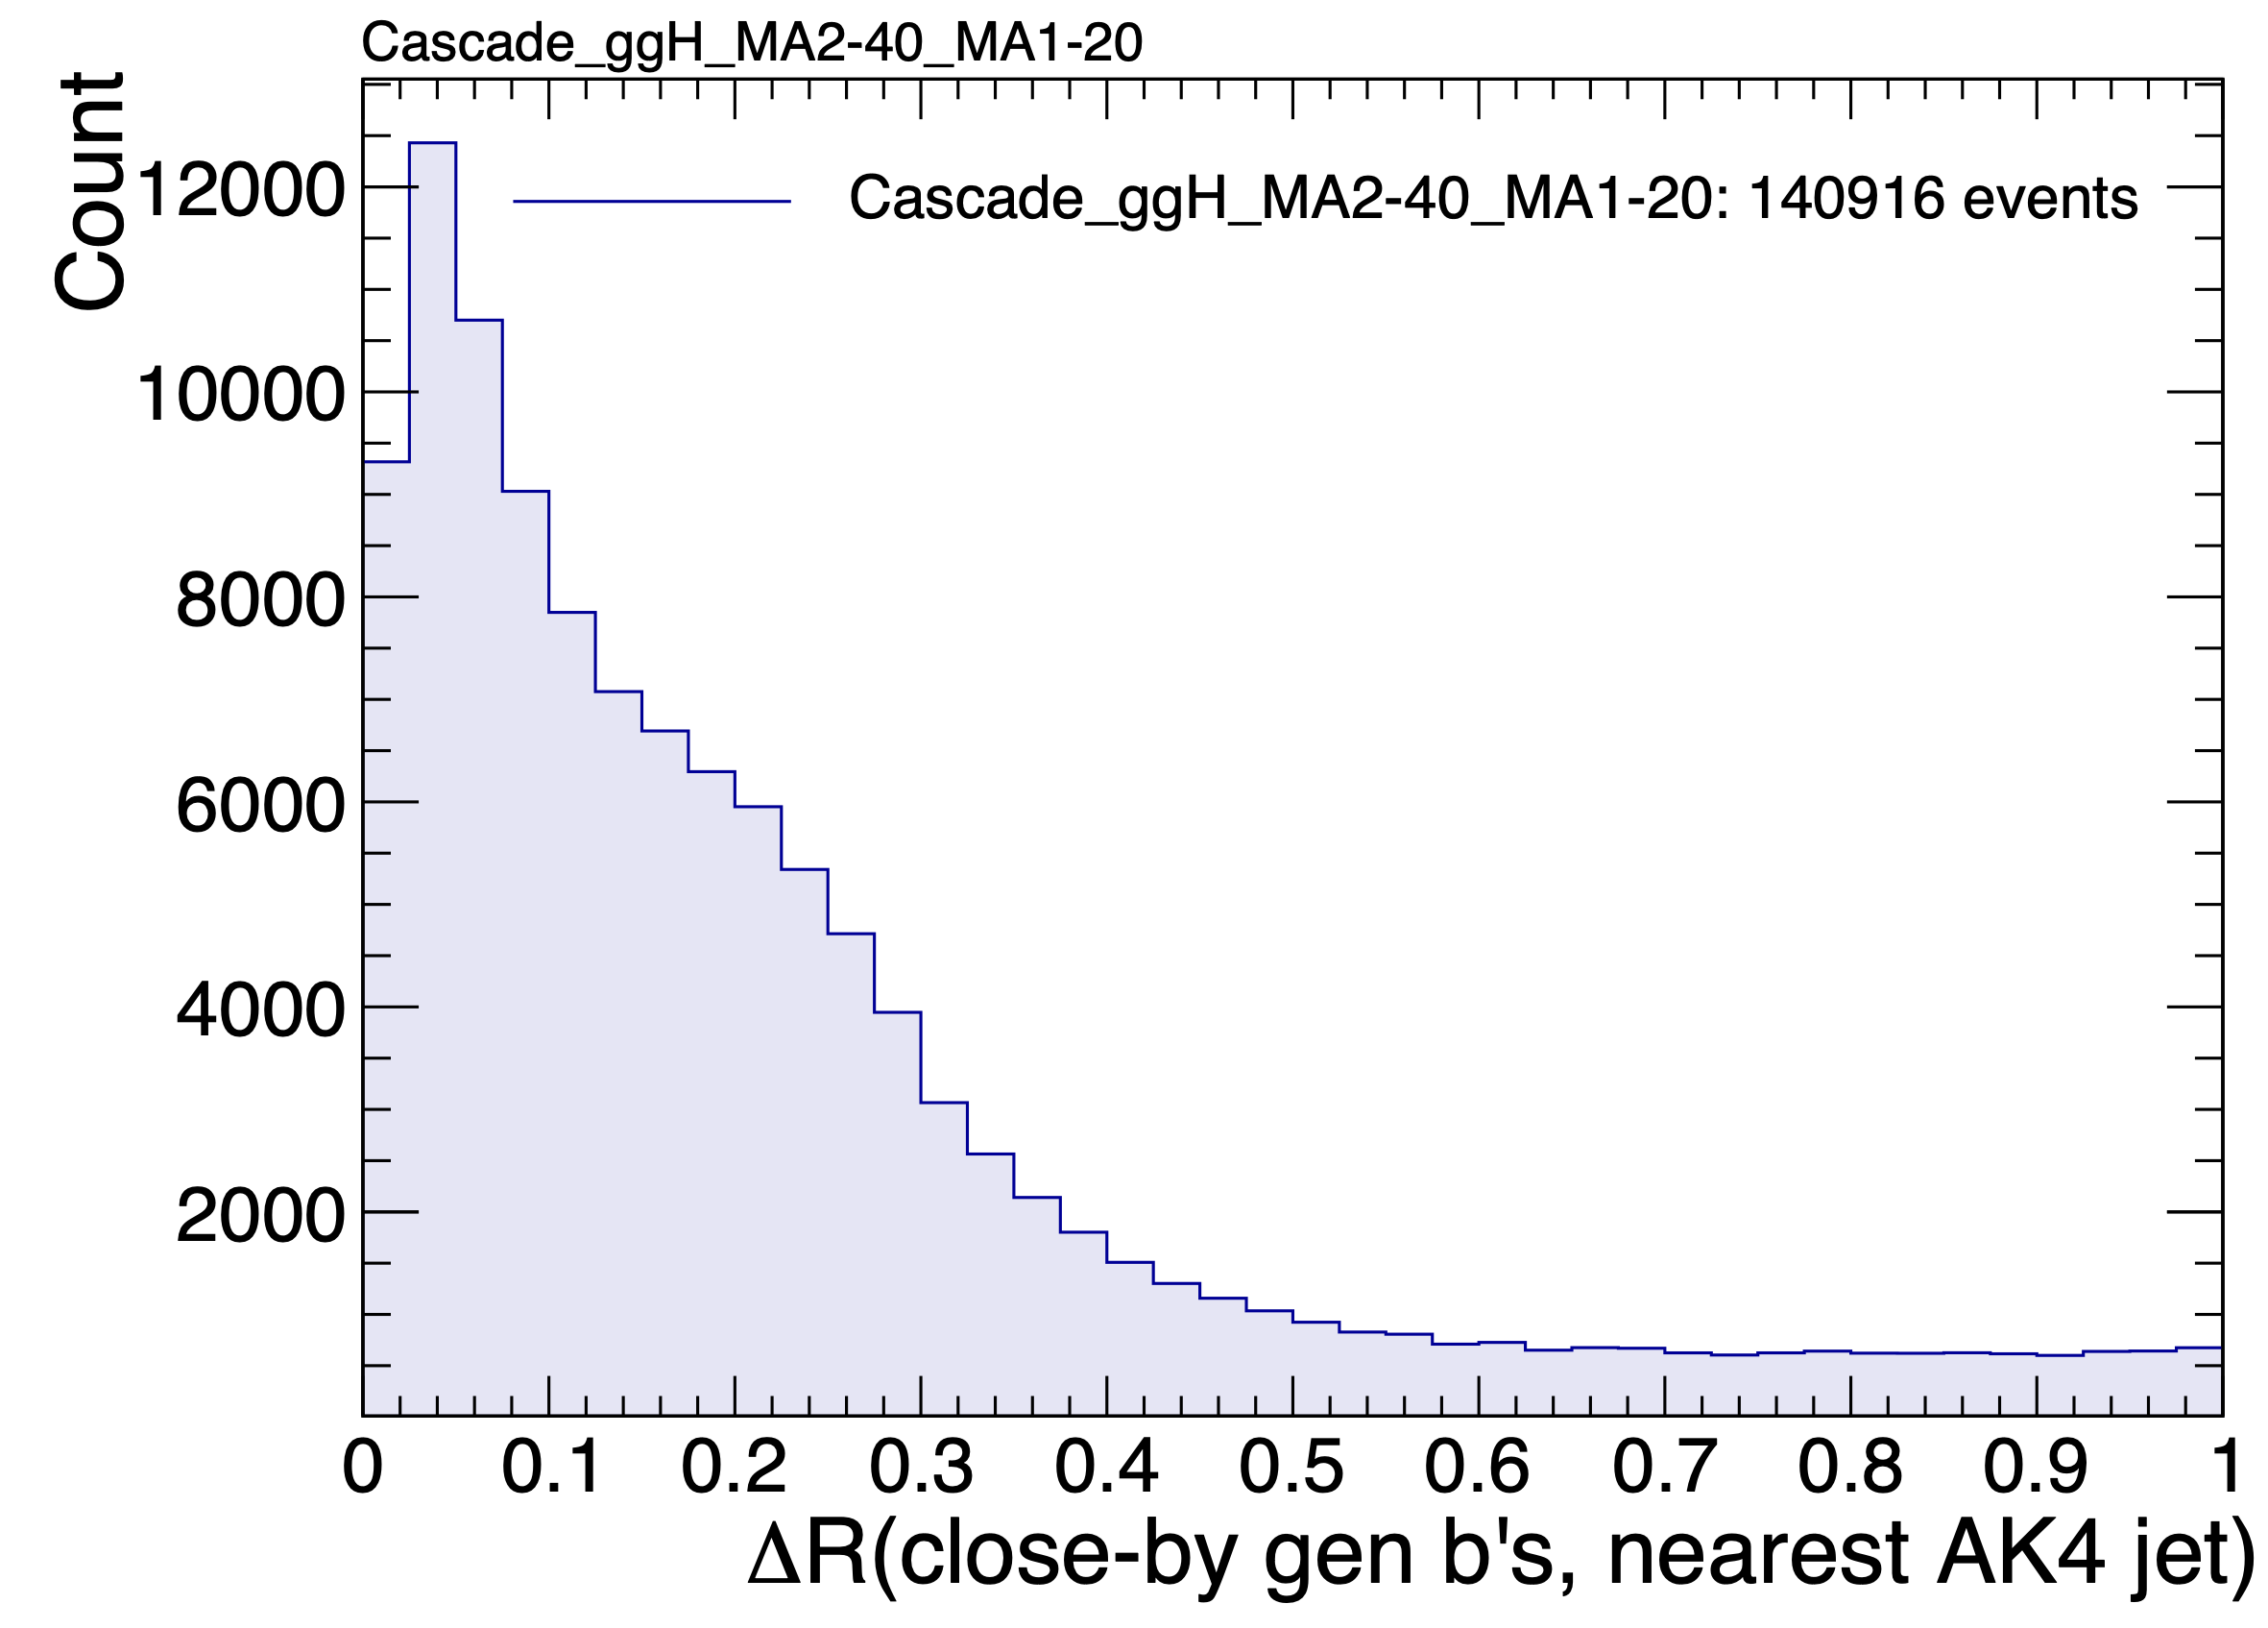
\includegraphics[width=1.0\textwidth]{figures/ch-11-asymmetric/Cascade_ggH_MA2-40_MA1-20_deltaR_ak4_leadingPair}
        % \caption{$\tau_{h}$ efficiency from $e\tau_{h}$ trigger.}
        % \label{fig:}
    \end{subfigure}     
    \caption{Distributions (arbitrary units) of transverse momentum $p_{T}$ resolution and $\Delta R$ between the two closest generator-level $b$ jets, treated as one object, and the nearest reconstructed AK4 jet, for two different $h\rightarrow a_1 a_2$ mass hypotheses $(m_{a_1}, m_{a_2}) = (100, 15)$ GeV (\textit{top left, top right}) and $(40, 20)$ GeV (\textit{bottom left, bottom right}) in the ggH production of the 125 GeV $h$. In the $(40, 20)$ GeV mass point, the longer $p_{T}$ resolution tail (\textit{bottom left}) indicates that the reconstructed jet underestimates the generator b-flavor jets' energy, and the significant fraction of events with larger $\Delta R$ values (\textit{bottom right}) indicate worse matching.}
    \label{fig:cascade_matching_to_AK4_jets}
\end{figure}



\section{Current control plots for \texorpdfstring{$\mu\tau_{h}$}{mutauh} channel}
\label{section:a1a2_control_plots}
The $\tau\tau$ states for the $h \rightarrow a_1 a_2$ to $4b2\tau$ analysis will be similar to those studied in $h\rightarrow aa \rightarrow bb\tau\tau$. For the $\mu\tau_{h}$ channel, histograms of the key kinematic variables are made for data and the sum of the expected backgrounds, which are estimated from Monte Carlo samples, embedded samples, and the data-driven method for estimating jets faking $\tau_{h}$ as described in Chapter \ref{chapter:ch-7:background-estimation}. Nominal values of the scale factors and event reweighing are applied, as described in Chapter \ref{chapter:ch-8:scale-factors-and-corrections}. The errors shown in the figures only include statistical errors and only several of the full set of systematic errors (only those associated with the lepton energy scales and $\tau_{h}$ identification efficiency, described in Sections \ref{sec:tau_energy_scale}, \ref{sec:muon_energy_scale}, and \ref{sec:tauh_id_efficiency}). 

The $p_{T}$, $\eta$, and $\phi$ of the leading muon and hadronic tau $\tau_{h}$, and the di-tau visible mass $m_{\text{vis}}$ and momentum $p_{T, \text{vis}}$, are shown in Fig. \ref{fig:nanoAOD_mutau_control_plots_leading_mutauh}. The $p_{T}$, $\eta$, and $\phi$ of the the leading and sub-leading b-tag jets, and the missing transverse energy magnitude and azimuthal direction, are shown in Fig. \ref{fig:nanoAOD_mutau_control_plots_btagjets_met_metphi}.

\begin{figure}[ht]
    \centering
    \begin{subfigure}{0.45\textwidth}
        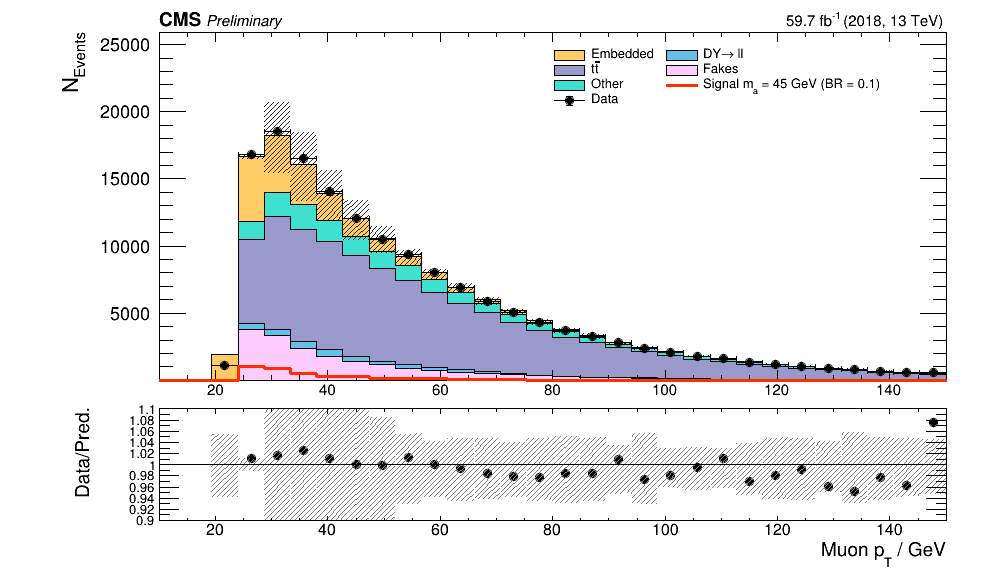
\includegraphics[width=1.0\textwidth]{figures/ch-11-asymmetric/mutau_pt_1.png}
    \end{subfigure}
    \hfill
    \begin{subfigure}{0.45\textwidth}
        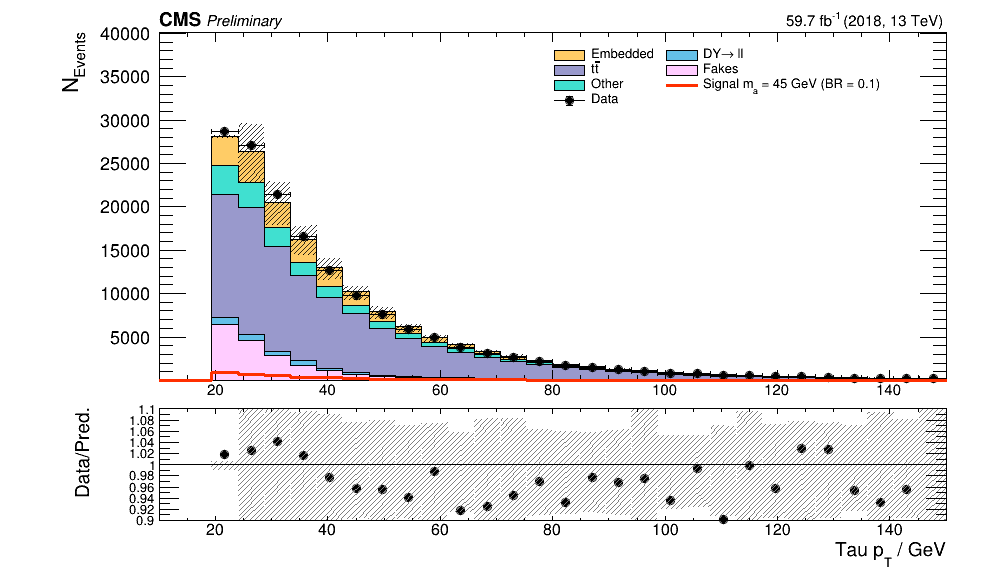
\includegraphics[width=1.0\textwidth]{figures/ch-11-asymmetric/mutau_pt_2.png}
    \end{subfigure} \\
    \begin{subfigure}{0.45\textwidth}
        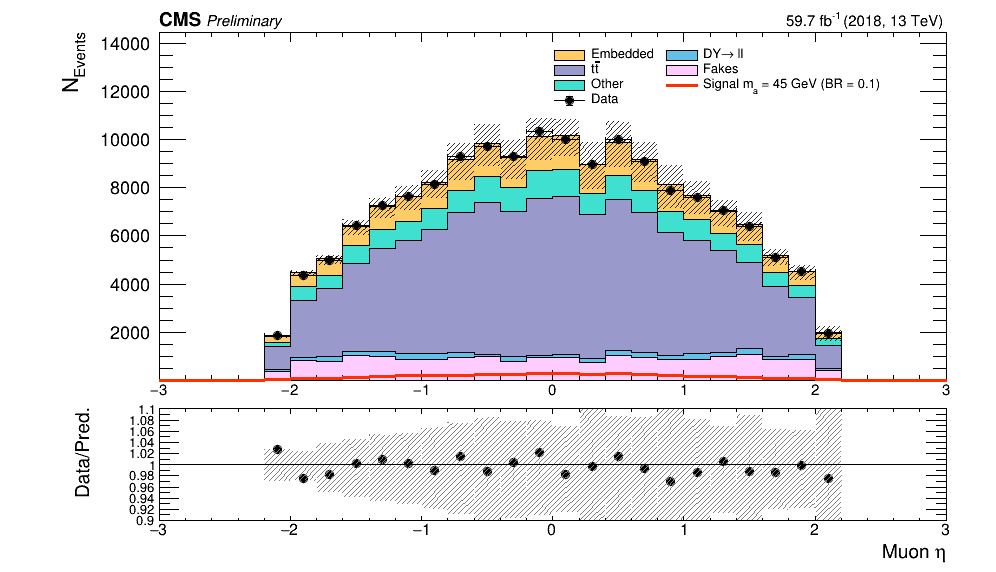
\includegraphics[width=1.0\textwidth]{figures/ch-11-asymmetric/mutau_eta_1.png}
    \end{subfigure}
    \hfill
    \begin{subfigure}{0.45\textwidth}
        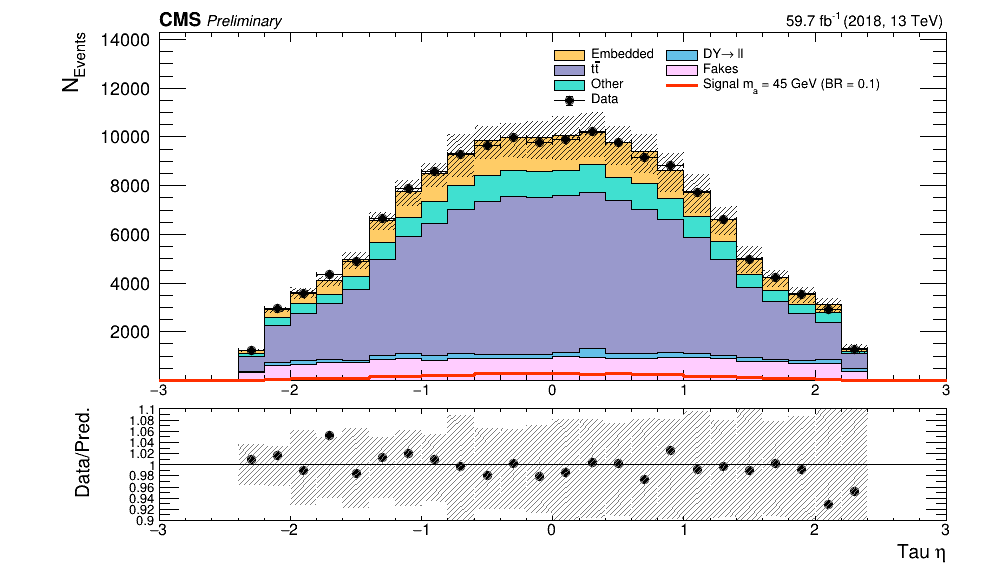
\includegraphics[width=1.0\textwidth]{figures/ch-11-asymmetric/mutau_eta_2.png}
    \end{subfigure} \\   
    \begin{subfigure}{0.45\textwidth}
        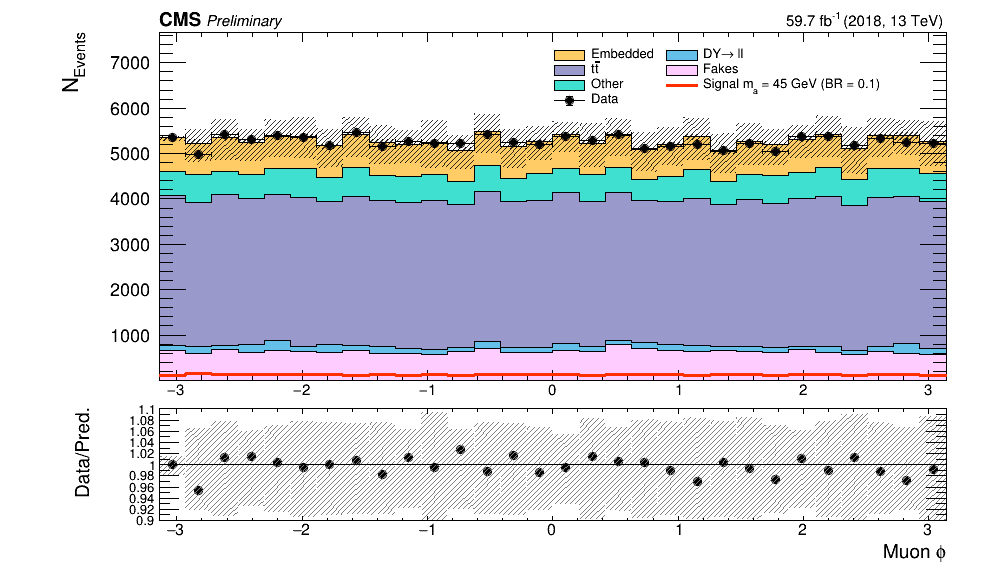
\includegraphics[width=1.0\textwidth]{figures/ch-11-asymmetric/mutau_phi_1.png}
    \end{subfigure}
    \hfill
    \begin{subfigure}{0.45\textwidth}
        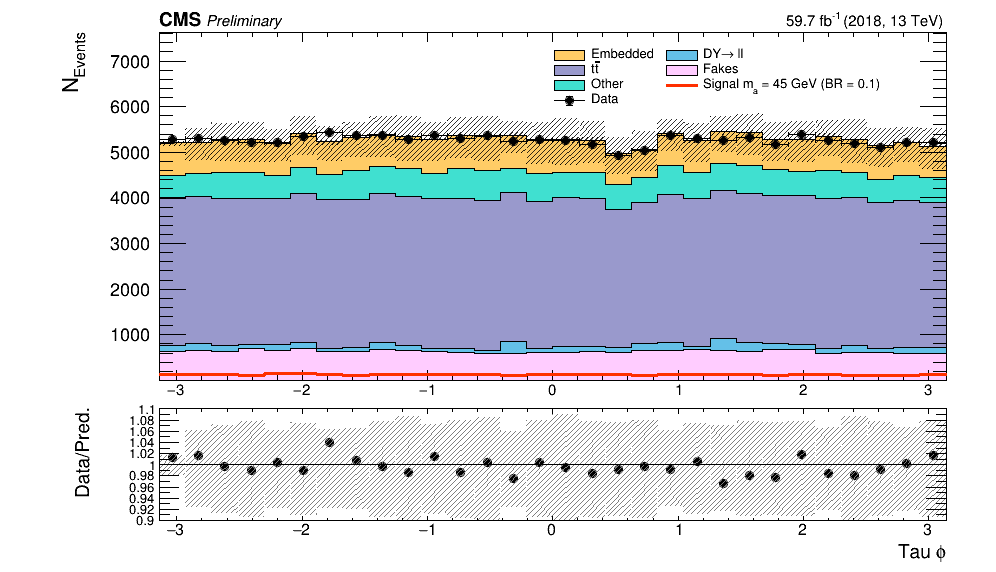
\includegraphics[width=1.0\textwidth]{figures/ch-11-asymmetric/mutau_phi_2.png}
    \end{subfigure} \\     
    \begin{subfigure}{0.45\textwidth}
        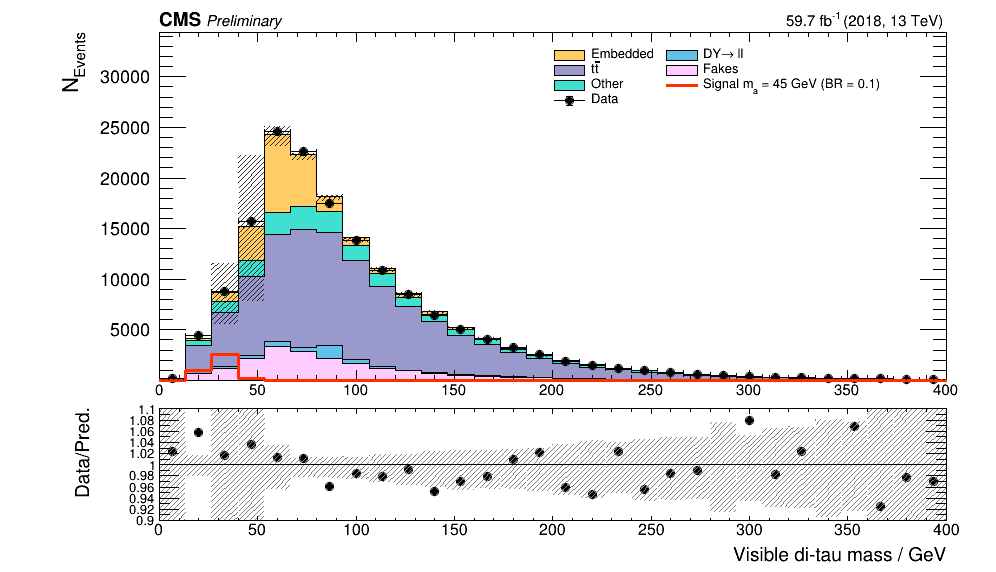
\includegraphics[width=1.0\textwidth]{figures/ch-11-asymmetric/mutau_m_vis.png}
    \end{subfigure}
    \hfill
    \begin{subfigure}{0.45\textwidth}
        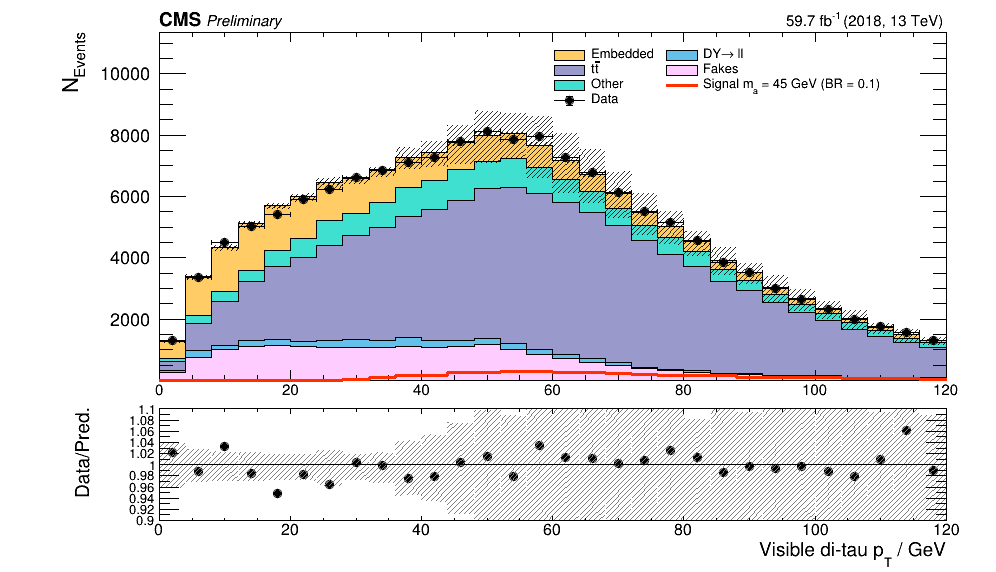
\includegraphics[width=1.0\textwidth]{figures/ch-11-asymmetric/mutau_pt_vis.png}
    \end{subfigure} \\   
    \caption{Kinematic properties of the leading muon and $\tau_{h}$ in the $\mu\tau_{h}$ channel: $p_T$ (\textit{top row}), $\eta$ (\textit{second row}), and $\phi$ (\textit{third row}). The visible 4-momenta of the muon and $\tau_{h}$ are summed, giving the visible di-tau mass $m_{\text{vis}}$ and transverse momentum $p_{T, \text{vis}}$.  The errors shown in the figures only include statistical errors and only several of the full set of systematic errors (only those associated with the lepton energy scales and $\tau_{h}$ identification efficiency).}
    \label{fig:nanoAOD_mutau_control_plots_leading_mutauh}
\end{figure}

\begin{figure}[ht]
    \centering
    \begin{subfigure}{0.45\textwidth}
        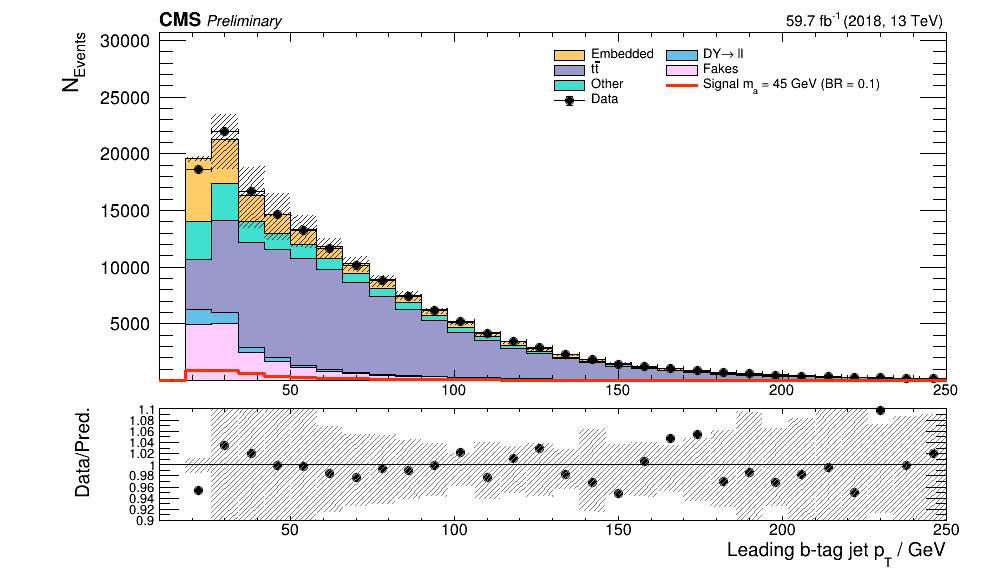
\includegraphics[width=1.0\textwidth]{figures/ch-11-asymmetric/mutau_bpt_deepflavour_1.png}
    \end{subfigure}
    \hfill
    \begin{subfigure}{0.45\textwidth}
        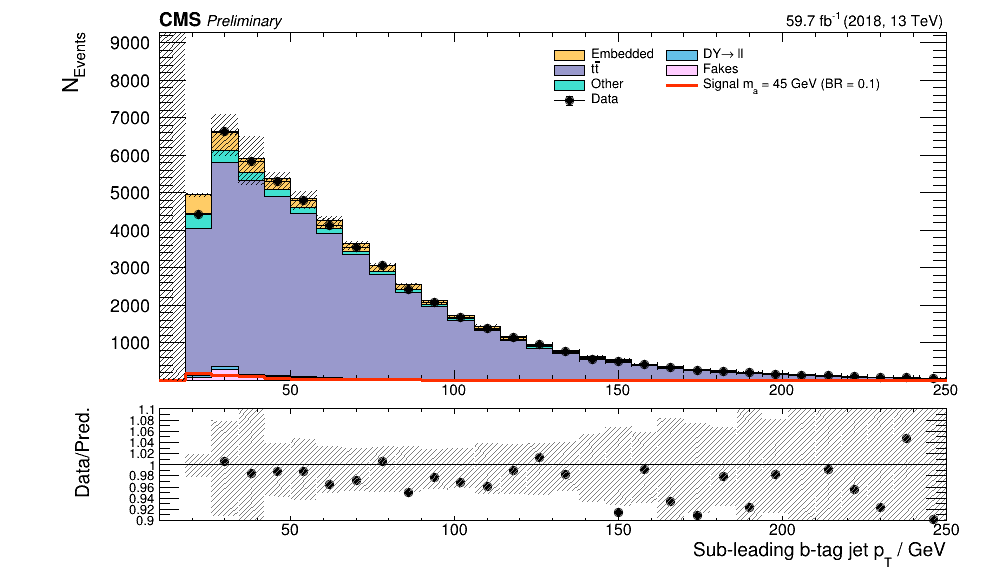
\includegraphics[width=1.0\textwidth]{figures/ch-11-asymmetric/mutau_bpt_deepflavour_2.png}
    \end{subfigure} \\
    \begin{subfigure}{0.45\textwidth}
        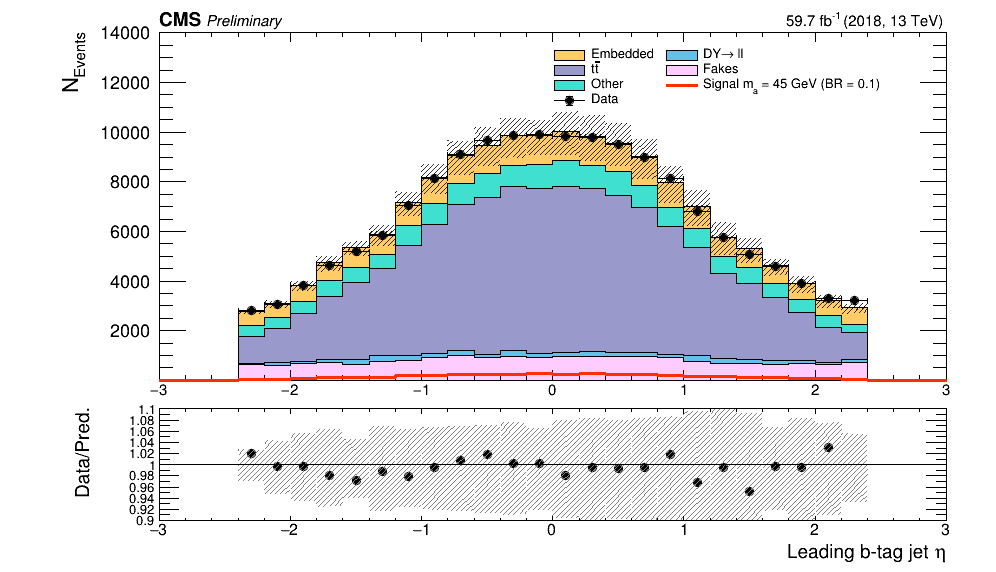
\includegraphics[width=1.0\textwidth]{figures/ch-11-asymmetric/mutau_beta_deepflavour_1.png}
    \end{subfigure}
    \hfill
    \begin{subfigure}{0.45\textwidth}
        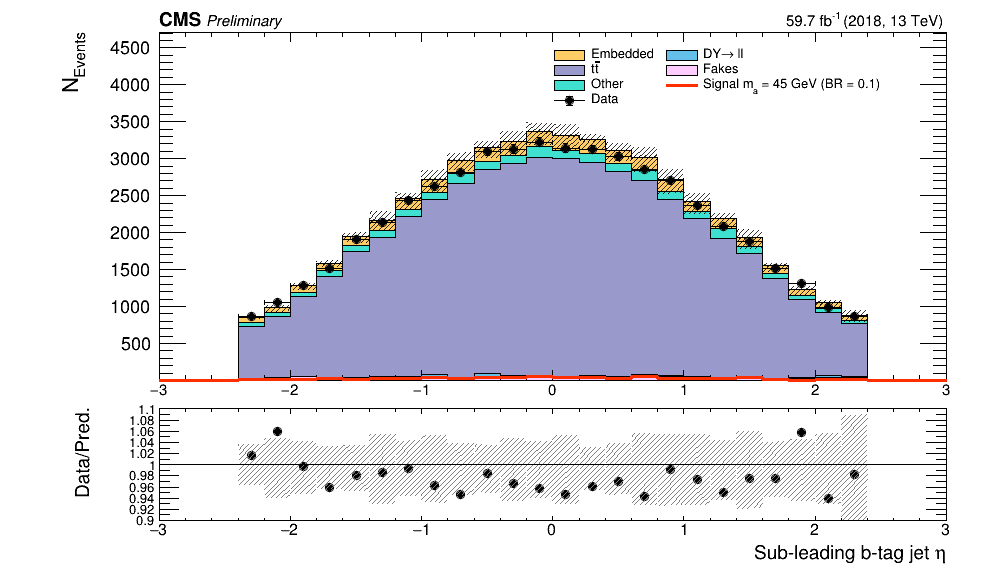
\includegraphics[width=1.0\textwidth]{figures/ch-11-asymmetric/mutau_beta_deepflavour_2.png}
    \end{subfigure} \\   
    \begin{subfigure}{0.45\textwidth}
        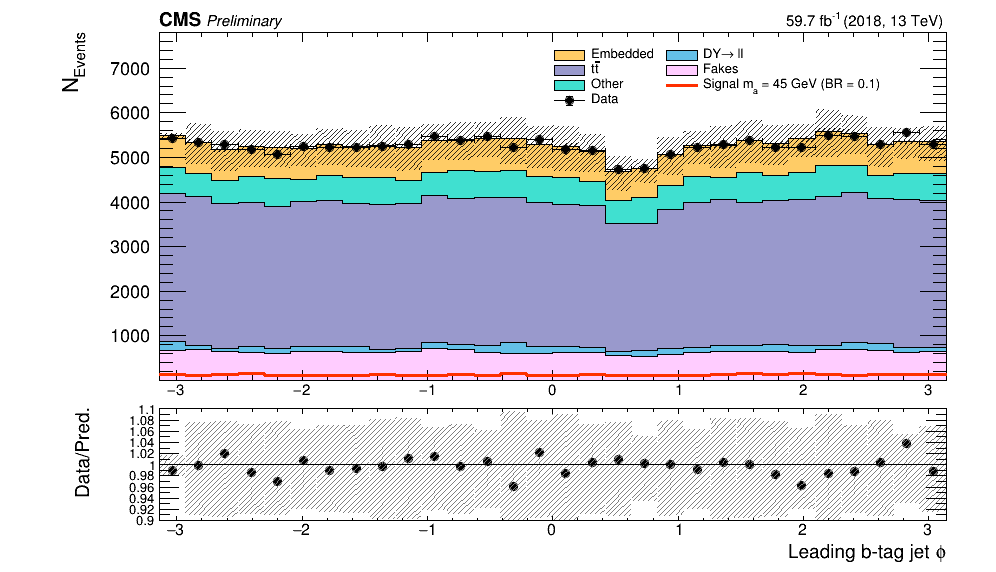
\includegraphics[width=1.0\textwidth]{figures/ch-11-asymmetric/mutau_bphi_deepflavour_1.png}
    \end{subfigure}
    \hfill
    \begin{subfigure}{0.45\textwidth}
        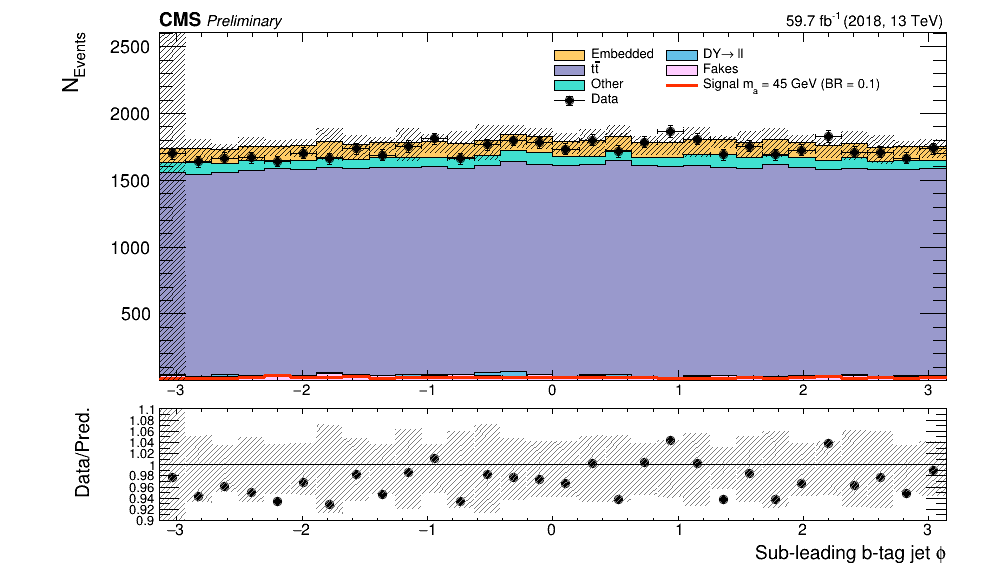
\includegraphics[width=1.0\textwidth]{figures/ch-11-asymmetric/mutau_bphi_deepflavour_2.png}
    \end{subfigure} \\     
    \begin{subfigure}{0.45\textwidth}
        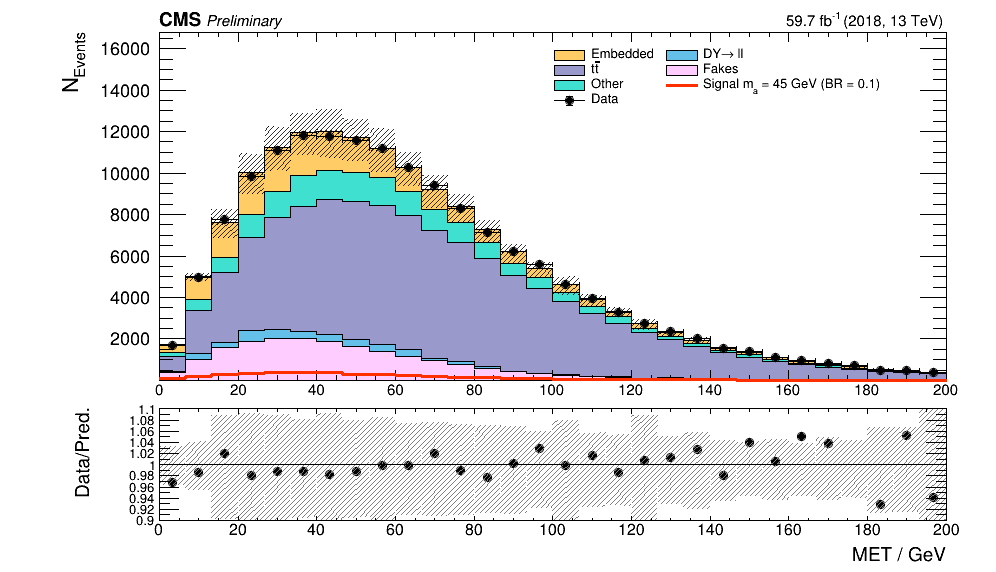
\includegraphics[width=1.0\textwidth]{figures/ch-11-asymmetric/mutau_met.png}
    \end{subfigure}
    \hfill
    \begin{subfigure}{0.45\textwidth}
        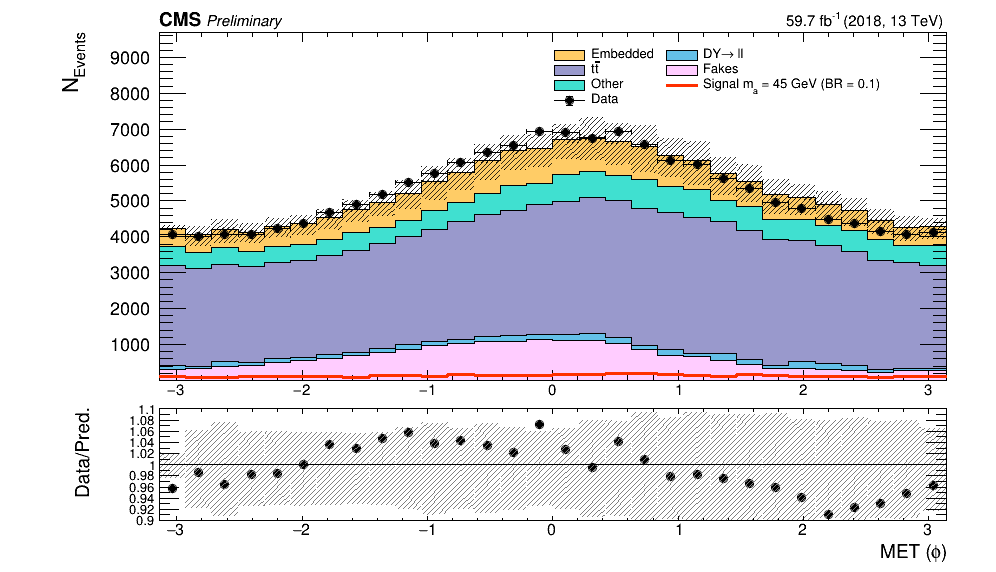
\includegraphics[width=1.0\textwidth]{figures/ch-11-asymmetric/mutau_metphi.png}
    \end{subfigure} \\   
    \caption{Kinematic properties of the leading and sub-leading b-tag jets in the $\mu\tau_{h}$ final state: jet $p_{T}$ (\textit{top row}), $\eta$ (\textit{second row}), $\phi$ (\textit{third row}), as well as the missing transverse energy magnitude and azimuthal direction (\textit{bottom row}). The errors shown in the figures only include statistical errors and only several of the full set of systematic errors (only those associated with the lepton energy scales and $\tau_{h}$ identification efficiency).}
    \label{fig:nanoAOD_mutau_control_plots_btagjets_met_metphi}
\end{figure}
